\subsection{Harmonic Oscillator}
The harmonic oscillator was used to evaluate the performance of different neural network architectures before applying them to more complex and demanding physical systems. Instead of investigating the influence of physical parameters, these experiments focused on evaluating different neural configurations by varying the number of hidden layers, the number of neurons per layer, and the learning rate, while keeping the physical system fixed.

\begin{table}[htbp]
\centering
\small
\begin{tabular}{ccccccc}
\toprule
Exp & 
\makecell{Learning\\Rate} & 
\makecell{Hidden\\Layers} & 
\makecell{Neurons\\per Layer} & 
MSE & 
MAE & 
\makecell{Maximum\\Error} \\
\midrule
1 & 0.001 & 3 & 64  & 0.000869 & 0.021611 & 0.075934 \\
2 & 0.001 & 3 & 128 & 0.000344 & 0.014924 & 0.051416 \\
3 & 0.001 & 3 & 256 & 0.016496 & 0.085416 & 0.334049 \\
4 & 0.0005 & 3 & 256 & 0.000046 & 0.005407 & 0.033024 \\
5 & 0.0005 & 3 & 128 & 0.000105 & 0.006760 & 0.045358 \\
6 & 0.0005 & 4 & 64  & 0.000110 & 0.008516 & 0.027999 \\
7 & 0.0005 & 4 & 128 & 0.001400 & 0.029866 & 0.088467 \\
8 & 0.001 & 4 & 128 & 0.000787 & 0.020596 & 0.087798 \\
\bottomrule
\end{tabular}
\caption{Neural network configurations evaluated for the harmonic oscillator.}
\label{tab:harmonic_architecture}
\end{table}

Table 1 summarises the performance obtained by the different neural network architectures tested. In general, the network achieved low prediction errors across the different configurations, demonstrating that even relatively simple fully connected architectures are capable of accurately learning the sinusoidal dynamics of the harmonic oscillator.

Increasing the network size did not always improve performance. For example, increasing the number of neurons per layer from 128 to 256 while maintaining the learning rate at $10^{-3}$ increased the MSE from $3.44\times10^{-4}$ to $1.65\times10^{-2}$, indicating that larger models can be more difficult to optimise under the same training conditions. However, reducing the learning rate to $5\times10^{-4}$ improved the performance, reducing the MSE to $4.6\times10^{-5}$ in experiment 4, which corresponds to the best performance achieved in these experiments.

Similarly, increasing the depth of the network did not consistently improve the results. Although some deeper architectures achieved competitive performance, they generally produced higher errors than the best-performing structure with three hidden layers. These observations suggest that, for a simple linear dynamical system such as the harmonic oscillator, increasing model complexity provides limited benefits once sufficient representational capacity has been reached.

Based on these experiments, the configuration consisting of three hidden layers with 128 neurons per layer, Tanh activation, and a learning rate of $5\times10^{-4}$ was selected as the baseline architecture for the remaining experiments. Although some configurations achieved slightly lower errors in individual cases, this model was chosen because it provided a consistent balance between prediction accuracy, training stability, and computational efficiency. The objective of this selection was not to identify the absolute optimal architecture, but rather to establish a reliable reference model for comparing the influence of different physical parameters on the learning process. This configuration achieved an MSE of $1.05\times10^{-4}$, an MAE of $6.76\times10^{-3}$, and a maximum prediction error of $4.54\times10^{-2}$.

\subsection{Damped Harmonic Oscillator}
Following the validation of the neural network architecture using the harmonic oscillator, the damped harmonic oscillator was introduced to evaluate the model’s ability to learn dissipative dynamics. Unlike the ideal harmonic oscillator, where the oscillation amplitude remains constant, the presence of the damping coefficient $(\beta)$ introduces an exponential decay in the oscillation amplitude, increasing the complexity of the underlying temporal pattern.

A total of 50 experiments were performed, evaluating ten different damping coefficients $(\beta = 0.1$ to 1) and repeating each configuration with five different random seeds. The neural network architecture and training parameters were kept fixed throughout all experiments according to the configuration selected in Section 3.1.
\begin{figure}[htbp]
\centering
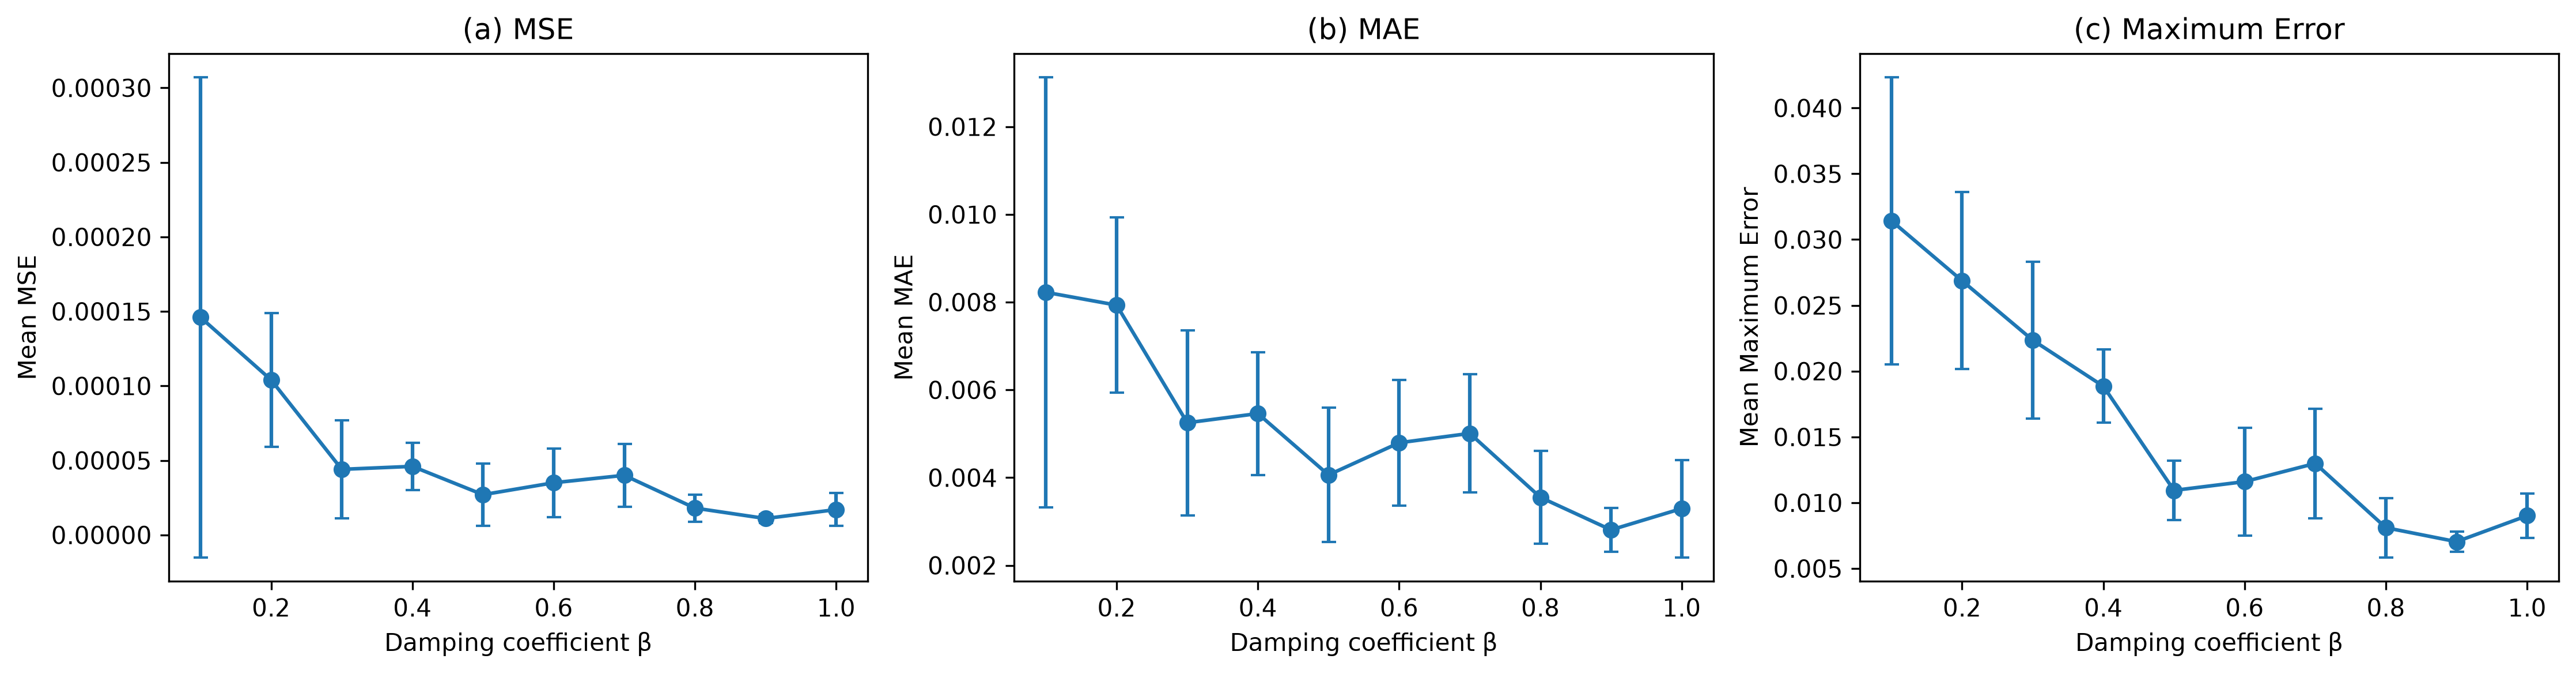
\includegraphics[width=0.8\textwidth]{figures/damped_harmonic_results.png}
\caption{\small Prediction error metrics for the damped harmonic oscillator across different damping coefficients. The figure shows the mean squared error (MSE), mean absolute error (MAE), and maximum prediction error obtained for each value of the damping coefficient.}
\label{fig:damped_harmonic_results}
\end{figure}

The obtained results are summarised in Figure 1, where the mean and standard deviation are shown for each damping coefficient. For all evaluated values, the network achieved consistently low approximation errors, demonstrating its ability to capture both the oscillatory behaviour and the amplitude decay.

For low damping values $(\beta < 0.3)$, the model exhibited slightly higher variability between random seeds. This behaviour can be attributed to the fact that the system remains closer to the undamped oscillator regime, where the network must accurately preserve long-lasting oscillations throughout the entire prediction interval. For example, at $(\beta = 0.1)$, the average MSE remained below $10^{-4}$, although some individual seeds produced larger errors.

As the damping coefficient increased, the model generally maintained stable performance. Between $(\beta = 0.4)$ and $(\beta = 1)$, the MSE remained consistently in the range of $10^{-5}$ to $10^{-4}$, while the maximum prediction error stayed below $4\times10^{-2}$ for almost all experiments. The lowest individual error was obtained for $(\beta = 0.8)$ with seed 2026, achieving an MSE of $3.98\times10^{-6}$ and a maximum error of $3.9\times10^{-3}$.

The influence of random initialisation was also limited. Although some configurations showed small variations between seeds, the overall trend remained unchanged, indicating that the learned representation was not strongly dependent on the initial network weights.

Furthermore, a clear decrease in prediction error can be observed as $\beta$ increases. Although the network already achieves accurate predictions for weakly damped systems, the average error progressively decreases with larger damping coefficients, reaching its lowest values as $\beta$ approaches 1.

This behaviour can be explained by the physical characteristics of the system. For small damping coefficients, the oscillator preserves its energy for longer periods, producing sustained oscillations that require the network to accurately predict the phase evolution over the entire simulation interval. Small deviations in the estimated frequency or phase accumulate over time, increasing the final prediction error.

In contrast, larger damping coefficients reduce the oscillation amplitude more rapidly, leading to smoother trajectories with lower long-term variability. Therefore, the neural network faces a simpler prediction task, as small deviations have a reduced impact on the final trajectory. This explains the observed reduction in MSE, MAE, and maximum error as the damping coefficient increases.

These results demonstrate that the neural network can successfully approximate damped oscillatory systems across a wide range of dissipation regimes. Compared with the harmonic oscillator, the additional exponential decay introduced by the damping term increases the complexity of the trajectory; however, the model maintains high prediction accuracy and stable generalisation performance.

\subsection{Forced Harmonic Oscillator}
The forced harmonic oscillator extends the damped harmonic oscillator by introducing a periodic external force. This additional term increases the complexity of the system, as the resulting motion depends on the interaction between the natural oscillation and the external excitation.

To evaluate this physical system, 65 experiments were performed, using 13 different values of the forcing angular frequency $(\Omega)$ and five different random seeds for each configuration. The reported metrics correspond to the average performance of the network for each value of $\Omega$, while the standard deviation was used to evaluate the stability of the training process.

Additionally, the coefficient of determination $(R^2)$ was included as an evaluation metric, defined as:
\begin{equation}
    R^2 = 1-\frac{\sum_{i=1}^{n}(y_i-\hat{y_i})^2}{\sum_{i=1}^{n}(y_i-\bar{y})^2}
\end{equation}

where $y_i$ represents the reference value, $\hat{y_i}$ represents the neural network prediction, $\bar{y}$ is the mean of the reference values, and $n$ is the number of samples.
\begin{figure}[htbp]
\centering
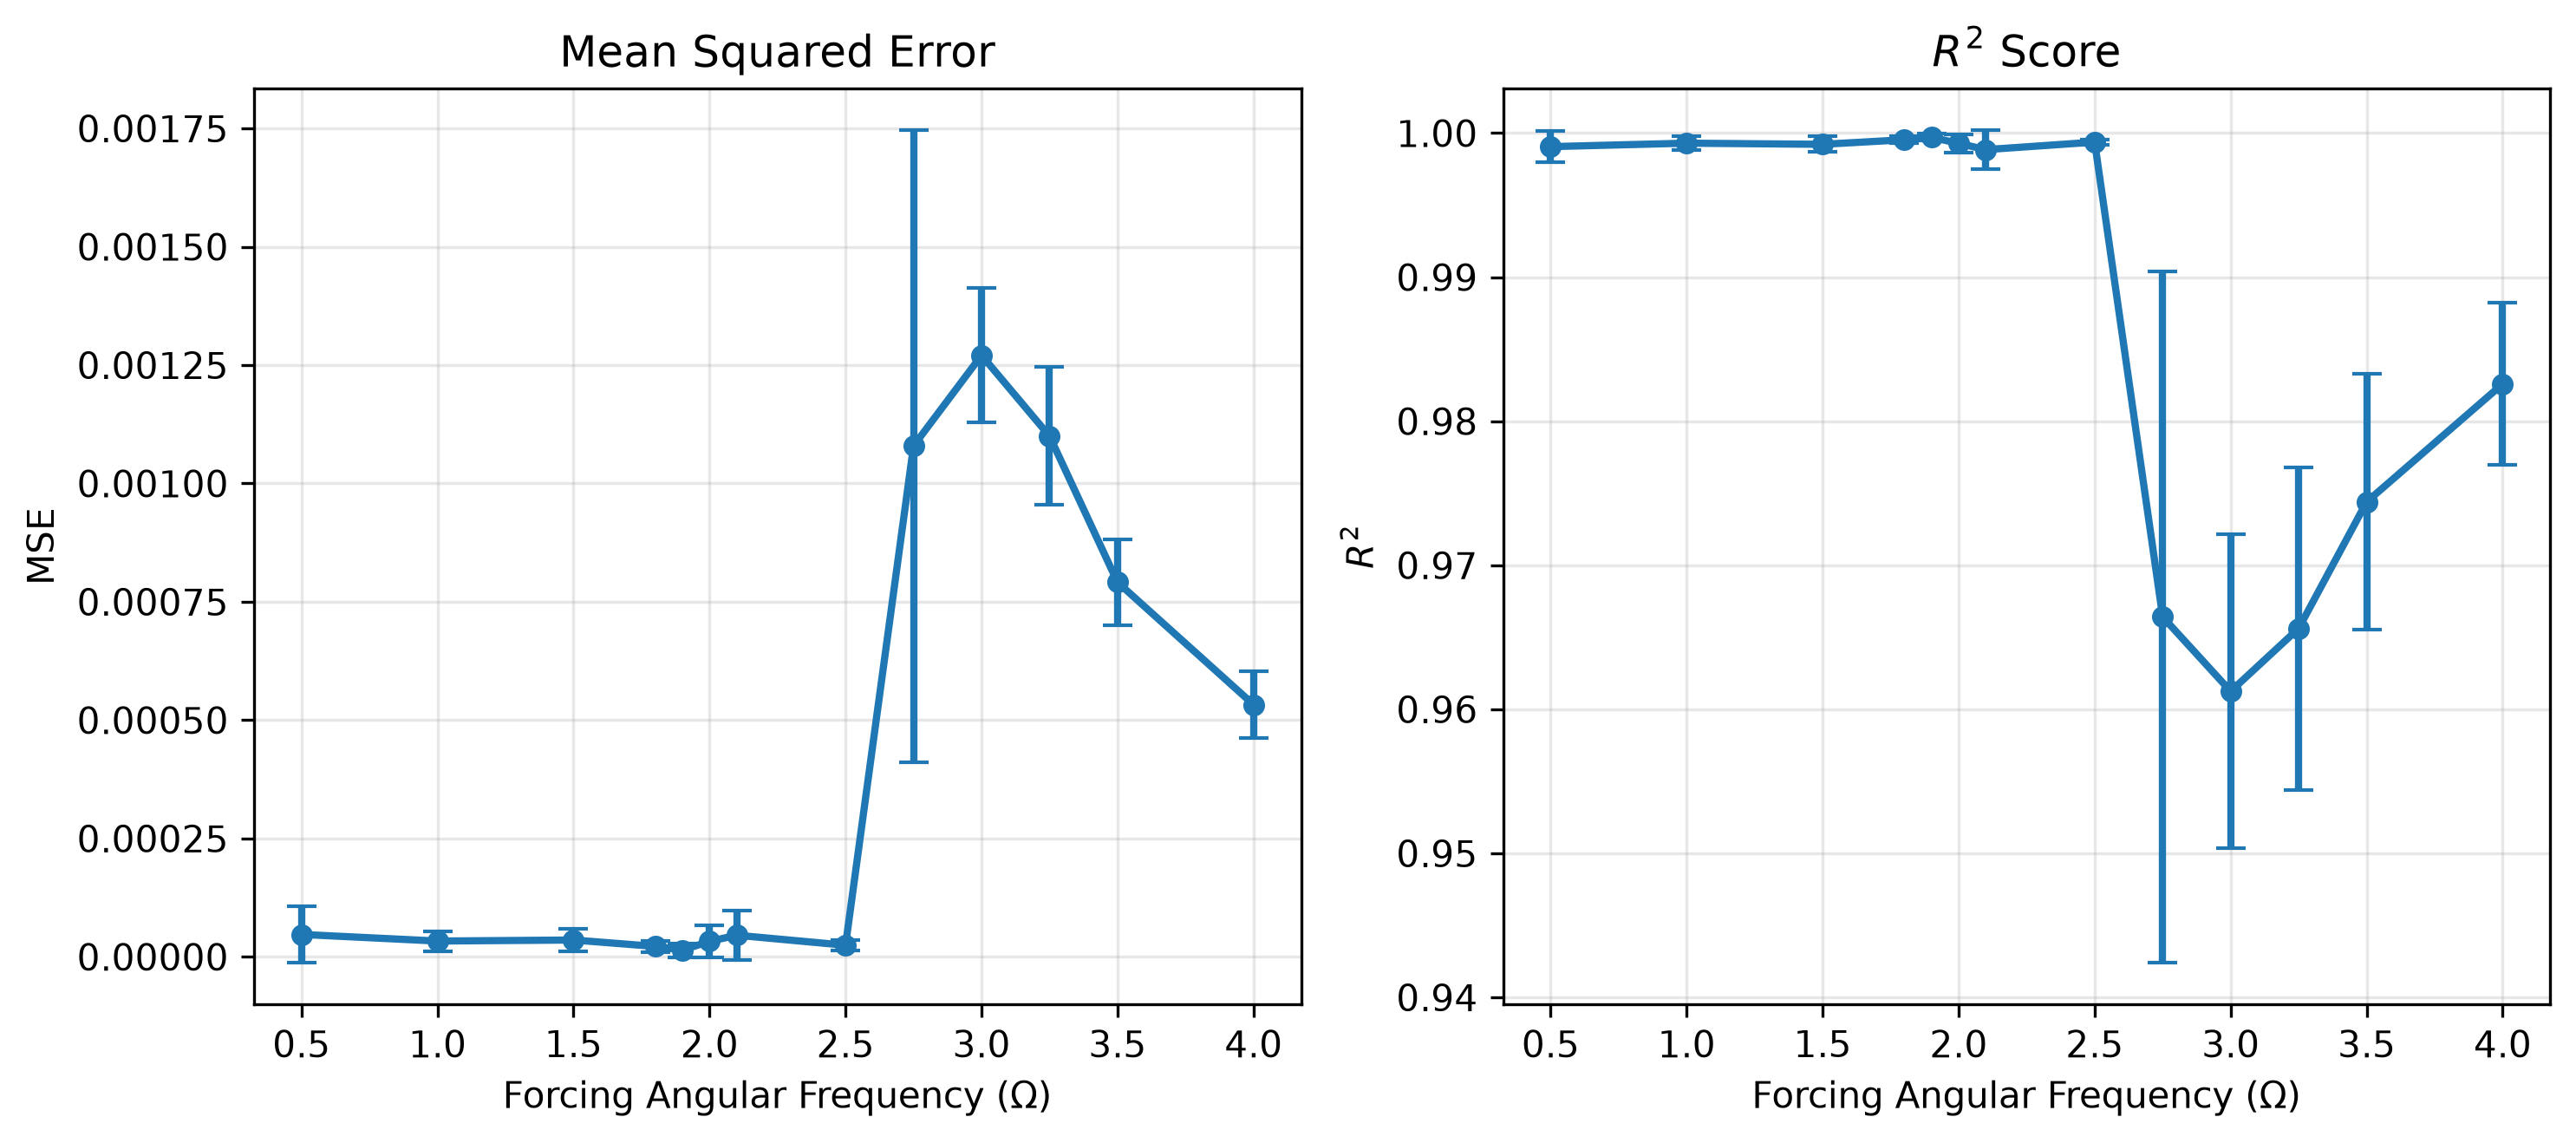
\includegraphics[width=0.8\textwidth]{figures/forcing_omega_results.png}
\caption{\small Prediction performance of the forced harmonic oscillator for different forcing angular frequencies. The figure shows the mean squared error (MSE) and coefficient of determination ($R^2$) obtained for each forcing frequency, including the variability across five independent training runs.}
\label{fig:forcing_omega_results}
\end{figure}

Figure 2 shows the results for both MSE and $(R^2)$. Each value of $(\Omega)$ includes its corresponding mean error and standard deviation. It can be observed that for forcing frequencies below approximately $(\Omega=2.5)$, the network achieved low approximation errors, whereas for higher frequencies the model began to show reduced prediction accuracy.

For example, for $(\Omega < 2.5)$, the highest average MSE was obtained at $(\Omega=0.5)$, with a value of $4.73\times10^{-5}$. Throughout this range, the MSE remained consistently close to zero, indicating stable prediction performance. The lowest individual error was obtained for $(\Omega=1.9)$ with seed 57, achieving an MSE of $2.03\times10^{-6}$.

However, when $(\Omega > 2.5)$, the network showed a decrease in prediction consistency. The lowest error in this regime, obtained at $(\Omega=4.0)$, was approximately eleven times larger than the highest error observed for $(\Omega < 2.5)$. The largest error occurred at $(\Omega=3.0)$, with an MSE of $1.2\times10^{-3}$. Unlike the lower-frequency regime, where the error remained stable, the prediction accuracy fluctuated as the forcing frequency increased.
\begin{figure}[htbp]
\centering
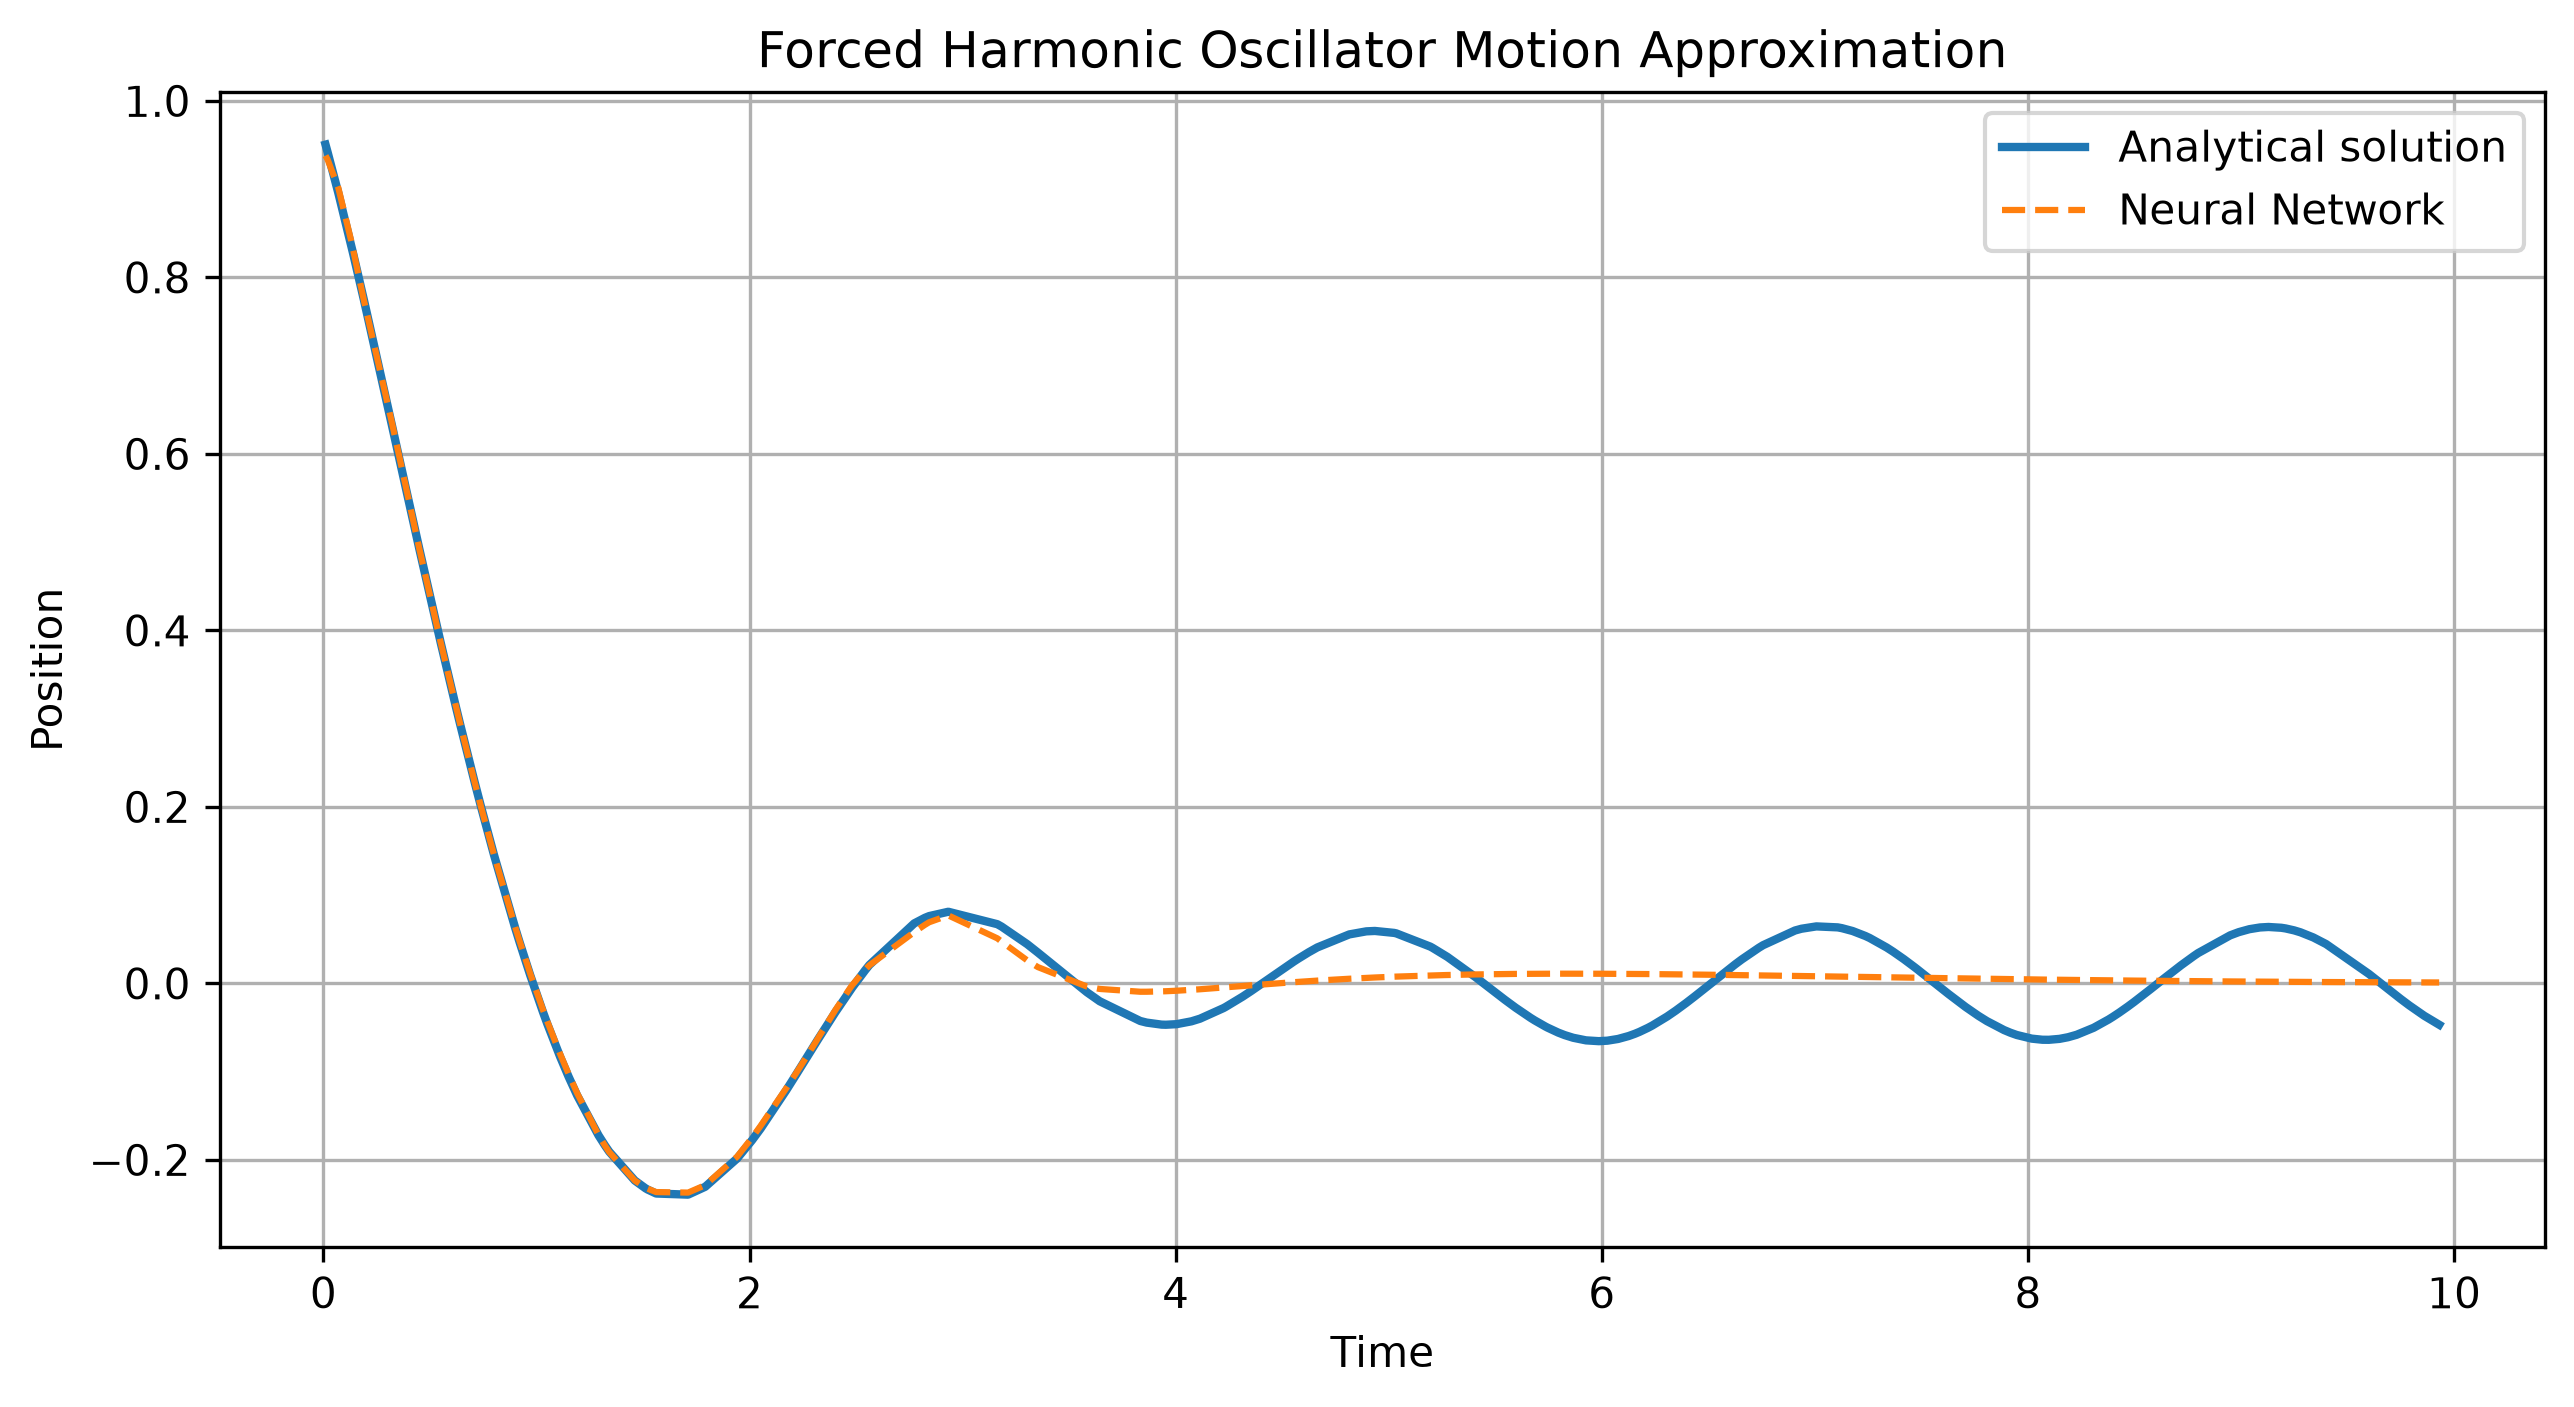
\includegraphics[width=0.8\textwidth]{figures/forced_harmonic_prediction.png}
\caption{\small Numerical solution and neural network prediction for the forced harmonic oscillator with forcing angular frequency $\Omega=3$ and random seed 42 over the simulation interval.}
\label{fig:forced_harmonic_prediction}
\end{figure}

Figure 3 shows the temporal evolution of the prediction error for the experiment with $(\Omega=3.0)$ and seed 42. It can be observed that, after approximately $(t=3)$, the neural network prediction deviates significantly from the reference trajectory, converging towards values close to zero.

The degradation in prediction accuracy observed for forcing frequencies above approximately $(\Omega=2.5)$ requires further analysis. Although the forced harmonic oscillator remains a deterministic system, the difficulty of the learning task is not determined exclusively by the complexity of the governing equation, but also by the characteristics of the generated trajectory and its suitability for approximation by the neural network.

The forced harmonic oscillator contains two distinct dynamical components: a transient response associated with the initial conditions and a stationary response \cite{landau1986mechanics} generated by the external excitation. The transient component decays exponentially according to $e^{-\beta t}$, becoming negligible after several seconds for the selected damping coefficient. However, during the initial stage of the trajectory, both components coexist, producing a signal composed of multiple oscillatory contributions.

For forcing frequencies close to the natural frequency of the oscillator, the resulting response remains relatively smooth \cite{taylor_classical_mechanics}, allowing the network to accurately approximate the trajectory. However, as the forcing frequency increases, the interaction between the natural dynamics and the external excitation produces more complex temporal patterns. The neural network must simultaneously learn the transient decay, the amplitude variation of the forced response, and the phase relationship between oscillations with different frequencies.

This effect becomes particularly relevant in the range $(\Omega=2.75-3.5)$, where the largest increase in prediction error is observed. In this regime, the trajectory combines relatively fast oscillations with a remaining transient contribution, creating a more challenging approximation problem. Since the model receives only the time variable as input, it does not have explicit information about the physical parameters and must infer the complete temporal relationship directly from the generated data.

Another possible contribution is related to the representational limitations of the multilayer perceptron architecture. Neural networks generally require more capacity to approximate high-frequency components compared with smoother, lower-frequency functions \cite{rahaman2019spectral}. Therefore, as the forcing frequency increases, the network may require additional complexity to represent the oscillatory structure with the same level of accuracy. The increase in error does not indicate physical instability of the oscillator, but rather that the selected architecture reaches a more challenging region of the function space.

Interestingly, the error does not increase indefinitely. For the highest tested frequency $(\Omega=4.0)$, the prediction accuracy improves compared with the intermediate-frequency regime. This suggests that the observed degradation is not caused solely by increasing oscillation frequency. Instead, it is likely related to the specific interaction between the transient and forced components within this frequency range. At larger frequencies, the transient contribution becomes relatively less significant compared with the forced oscillation, resulting in a simpler and more regular trajectory that can again be approximated more effectively by the neural network.

Further experiments with different architectures or longer simulation intervals would be required to isolate the contribution of each factor.

\subsection{Duffing Oscillator}
The Duffing oscillator represents the first nonlinear dynamical system investigated in this work. Unlike the previous oscillators, where the restoring force is proportional to the displacement, the Duffing equation introduces a nonlinear term that modifies the system response. This introduces additional complexity to the dynamics and provides a more challenging scenario for neural network prediction.

The system is defined by Equation~\ref{eq:duffing_oscillator}, where the cubic term introduces nonlinear behaviour \cite{strogatz2015nonlinear} and allows the system to exhibit complex phenomena such as amplitude-dependent oscillations and sensitivity to parameter variations \cite{strogatz2015nonlinear}.

The neural network architecture and training procedure were kept identical to those used in the previous experiments. The objective of this experiment was to evaluate whether the model, previously validated on linear systems, could successfully approximate nonlinear dynamics without requiring modifications to its structure.
\begin{figure}[htbp]
\centering
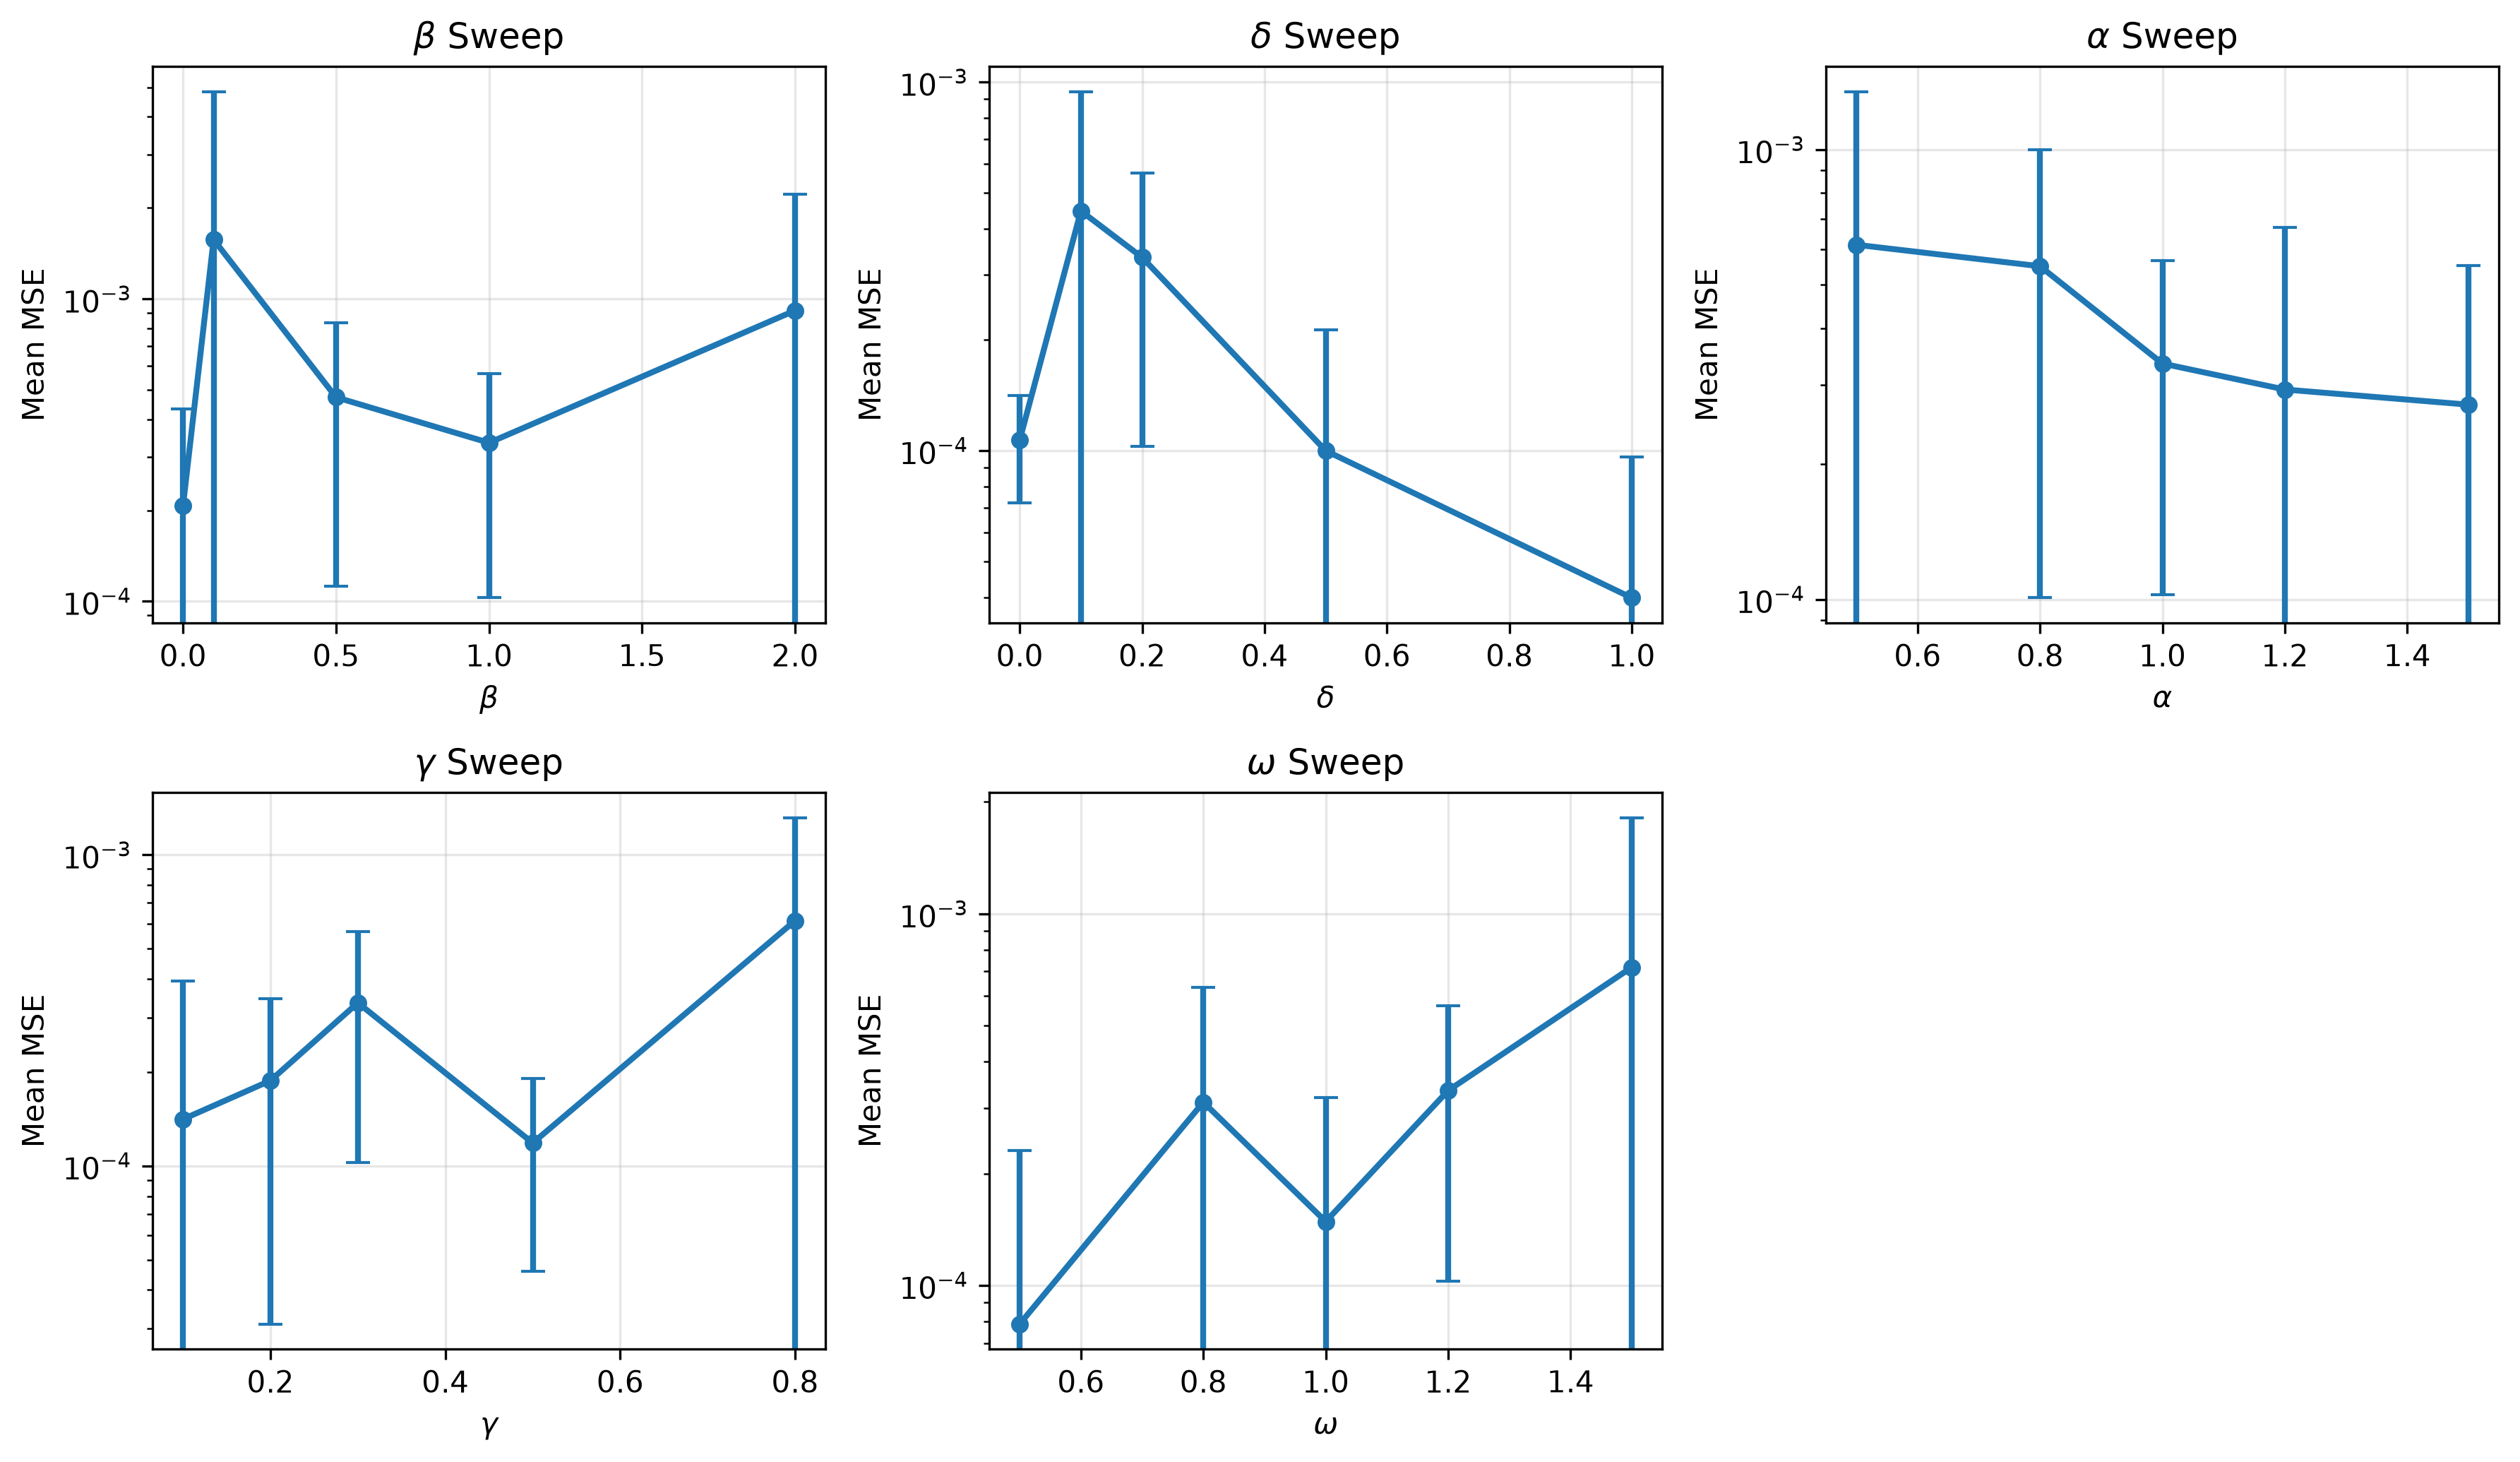
\includegraphics[width=0.8\textwidth]{figures/duffing_all_sweeps.png}
\caption{\small Mean squared error (MSE) of the Duffing oscillator for different parameter variations. The five subplots correspond to independent sweeps of the damping coefficient ($\delta$), linear stiffness ($\alpha$), nonlinear stiffness ($\beta$), forcing amplitude ($\gamma$), and forcing frequency ($\Omega$), with results averaged over five random seeds.}
\label{fig:duffing_all_sweeps}
\end{figure}

The Duffing oscillator was evaluated through five independent parameter sweeps, one for each selected system parameter. For each sweep, five different parameter values were tested using five different random seeds, resulting in 25 training experiments per parameter. Figure 4 presents the mean MSE obtained for each explored parameter value, together with the variability caused by different training initialisations.

Unlike the previous experiments, no clear monotonic relationship was observed between the Duffing parameters and the prediction error. Although certain parameter values produced larger errors in individual executions, these variations were not consistent across different random seeds, suggesting that the observed differences are mainly related to training variability rather than a systematic increase in the difficulty of the learning task.

This behaviour indicates that, within the explored parameter range, modifying the Duffing parameters alone does not significantly increase the complexity of the prediction problem. Although the cubic restoring force introduces nonlinear dynamics and changes the system response, the resulting trajectories remain sufficiently smooth and regular for the neural network to approximate them accurately.

Therefore, the presence of nonlinear terms alone does not necessarily imply a significant degradation in predictive performance. Instead, these results suggest that the effective complexity of the generated trajectory is a more relevant factor than the mere presence of nonlinear terms in the governing equation.

\subsection{Simple Pendulum}
The simple pendulum represents a nonlinear physical system widely used as a benchmark for dynamical modelling. Unlike the harmonic oscillator, where the restoring force is proportional to the displacement, the restoring force of a pendulum depends on the sine of the angular position, resulting in nonlinear oscillatory behaviour for large amplitudes.
The system is described by Equation~\ref{eq:simple_pendulum}, where $g$ represents the gravitational acceleration and $L$ the pendulum length. For small angular displacements, the approximation $(\sin(\theta)\approx\theta)$ can be applied \cite{taylor_classical_mechanics}, reducing the system to a linear harmonic oscillator:
\begin{equation}
    \ddot{\theta}+\frac{g}{L}\theta=0
\end{equation}

To evaluate the behaviour of the neural network on this physical system, five different parameter sweeps were performed. In the first sweep, the simulation duration was used as the variable parameter, with five experiments performed using the same random seed.
\begin{figure}[htbp]
\centering
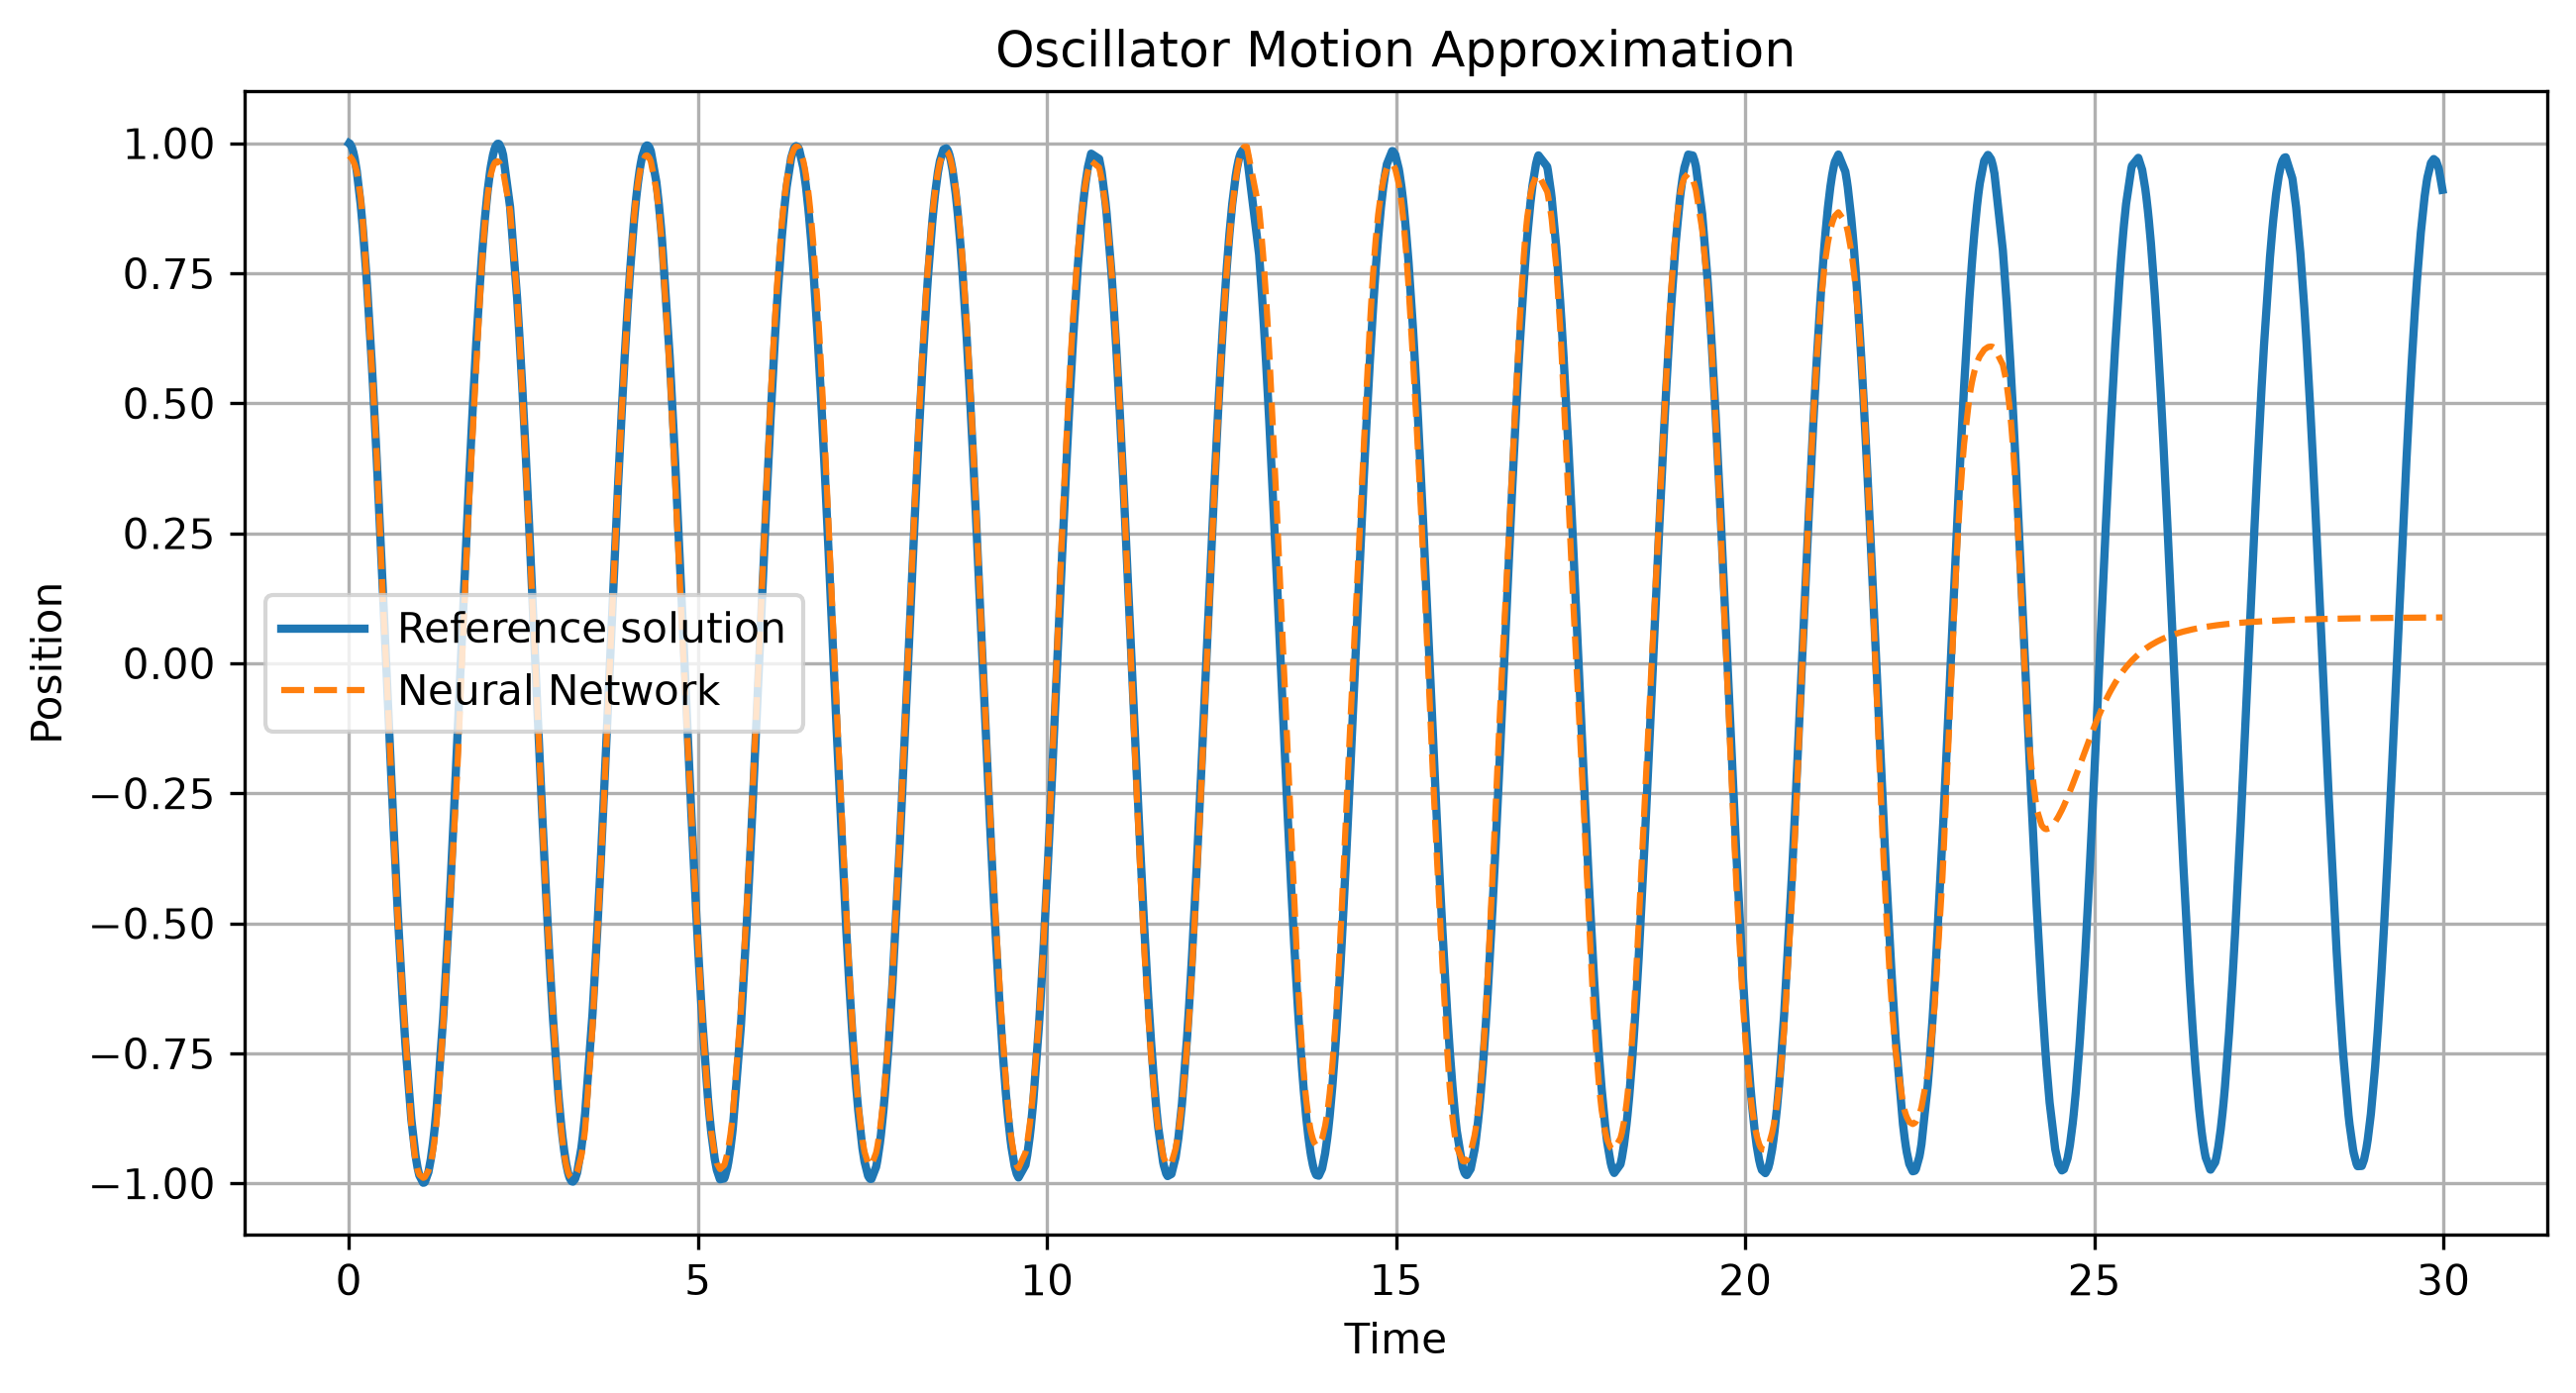
\includegraphics[width=0.8\textwidth]{figures/pendulum_prediction.png}
\caption{\small Numerical solution and neural network prediction for the simple pendulum over a 30-second simulation interval. The experiment was performed using random seed 42 and illustrates the long-term prediction behaviour of the model.}
\label{fig:pendulum_prediction}
\end{figure}

Figure 5 shows the experiment with a duration of 30 seconds and seed 42. The network accurately predicts the pendulum angle during most of the simulation interval. However, at approximately $(t=24)$ seconds, the prediction begins to deviate significantly, and the network loses the ability to reproduce the oscillatory behaviour accurately. Similar behaviour was observed for the 20-second experiment, while simulations with shorter durations maintained accurate predictions. Therefore, a duration of 10 seconds was selected for the remaining sweeps in order to avoid long-term error accumulation while still providing sufficient trajectory information.
\begin{figure}[htbp]
\centering
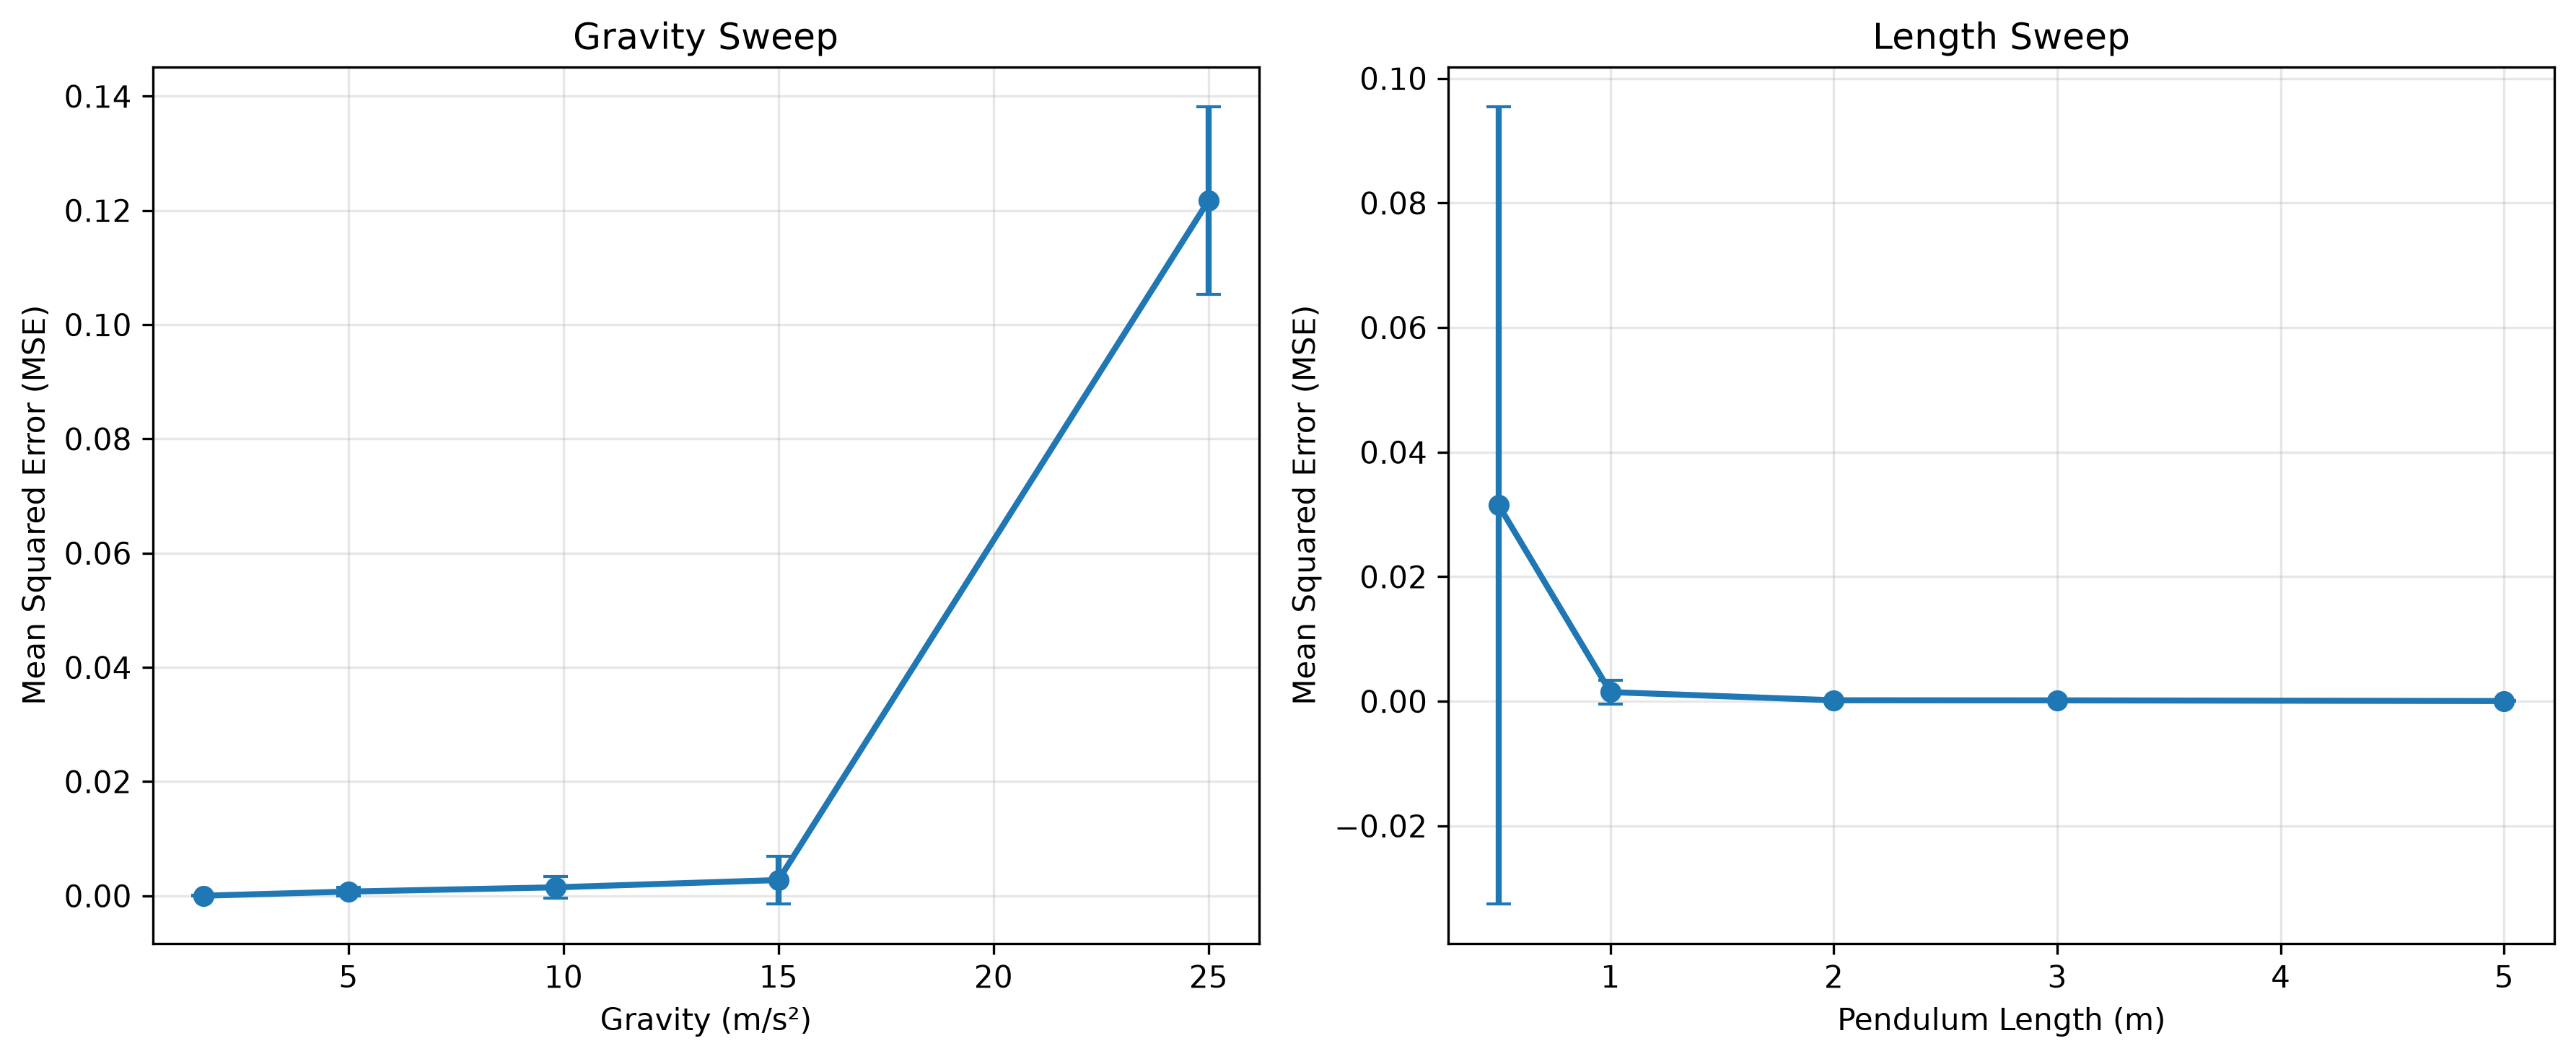
\includegraphics[width=0.8\textwidth]{figures/gravity_length_mse.png}
\caption{\small Mean squared error (MSE) of the simple pendulum for variations in gravitational acceleration ($g$) and pendulum length ($L$). The left subplot corresponds to the gravity sweep, while the right subplot corresponds to the length sweep. Results are averaged over five random seeds.}
\label{fig:gravity_length_mse}
\end{figure}

The next sweep investigated the effect of gravitational acceleration. This experiment contained five different gravity values and five random seeds per value, resulting in a total of 25 experiments. Figure 6 (left) shows the average MSE obtained for each gravitational acceleration.

For $(g<15)$, the MSE gradually increases but remains relatively low and consistent. However, for $(g=25)$, the neural network fails to approximate the dynamics accurately, reaching an average MSE of 0.12.

This behaviour can be explained by the dependence of the pendulum natural frequency on gravity. For small oscillations, the natural frequency is given by:
\begin{equation}
   \omega_0=\sqrt{\frac{g}{L}} 
   \label{eq:frequency}
\end{equation}

Therefore, increasing the gravitational acceleration increases the oscillation frequency. As observed in previous experiments with higher-frequency systems, the neural network shows greater difficulty representing faster temporal variations.

The length sweep followed the same structure, containing five different pendulum lengths with five random seeds each. Figure 6 (right) presents the average MSE for each length value. A behaviour similar to the gravity sweep can be observed, but in the opposite direction, since decreasing the pendulum length increases the natural frequency according to Equation~\ref{eq:frequency}.

\begin{figure}[htbp]
\centering
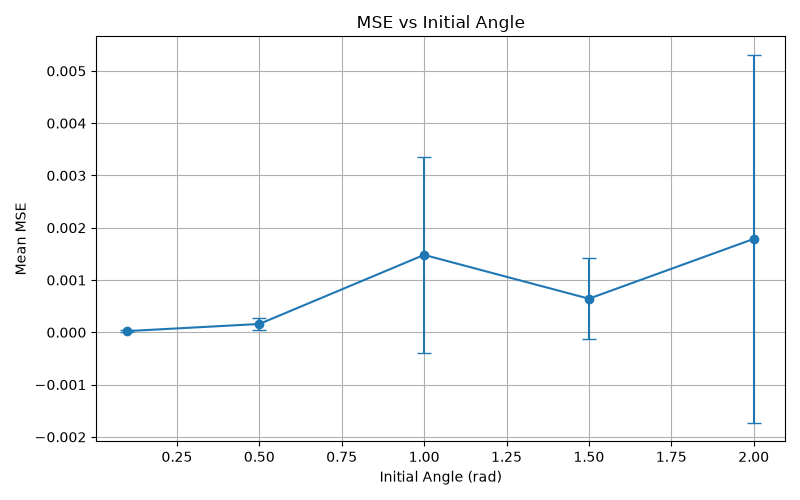
\includegraphics[width=0.8\textwidth]{figures/mse_vs_initial_angle.png}
\caption{\small Prediction error of the simple pendulum for different initial angular displacements ($\theta_0$). The figure shows the mean squared error (MSE) obtained for each value of the initial angle, averaged over five random seeds.}
\label{fig:mse_vs_initial_angle}
\end{figure}

The initial angle sweep also consisted of 25 experiments, with five initial angles evaluated using five random seeds each. Figure 7 shows the average MSE for each initial angle.

The results show no clear monotonic relationship between the initial angle and prediction error. If the difficulty of the learning problem depended only on the degree of nonlinearity, a continuous increase in MSE would be expected as the initial angle increases, since larger angles produce a stronger deviation from the small-angle approximation. However, although the lowest angles present slightly lower errors, no significant increase in error is observed for larger initial angles.

These results suggest that nonlinearity alone is not sufficient to explain prediction error. Although increasing the initial angle makes the governing equation depart further from the linear approximation, the resulting trajectories remain smooth and periodic within the simulated time interval. Consequently, the multilayer perceptron remains capable of accurately approximating the solution.
\begin{figure}[htbp]
\centering
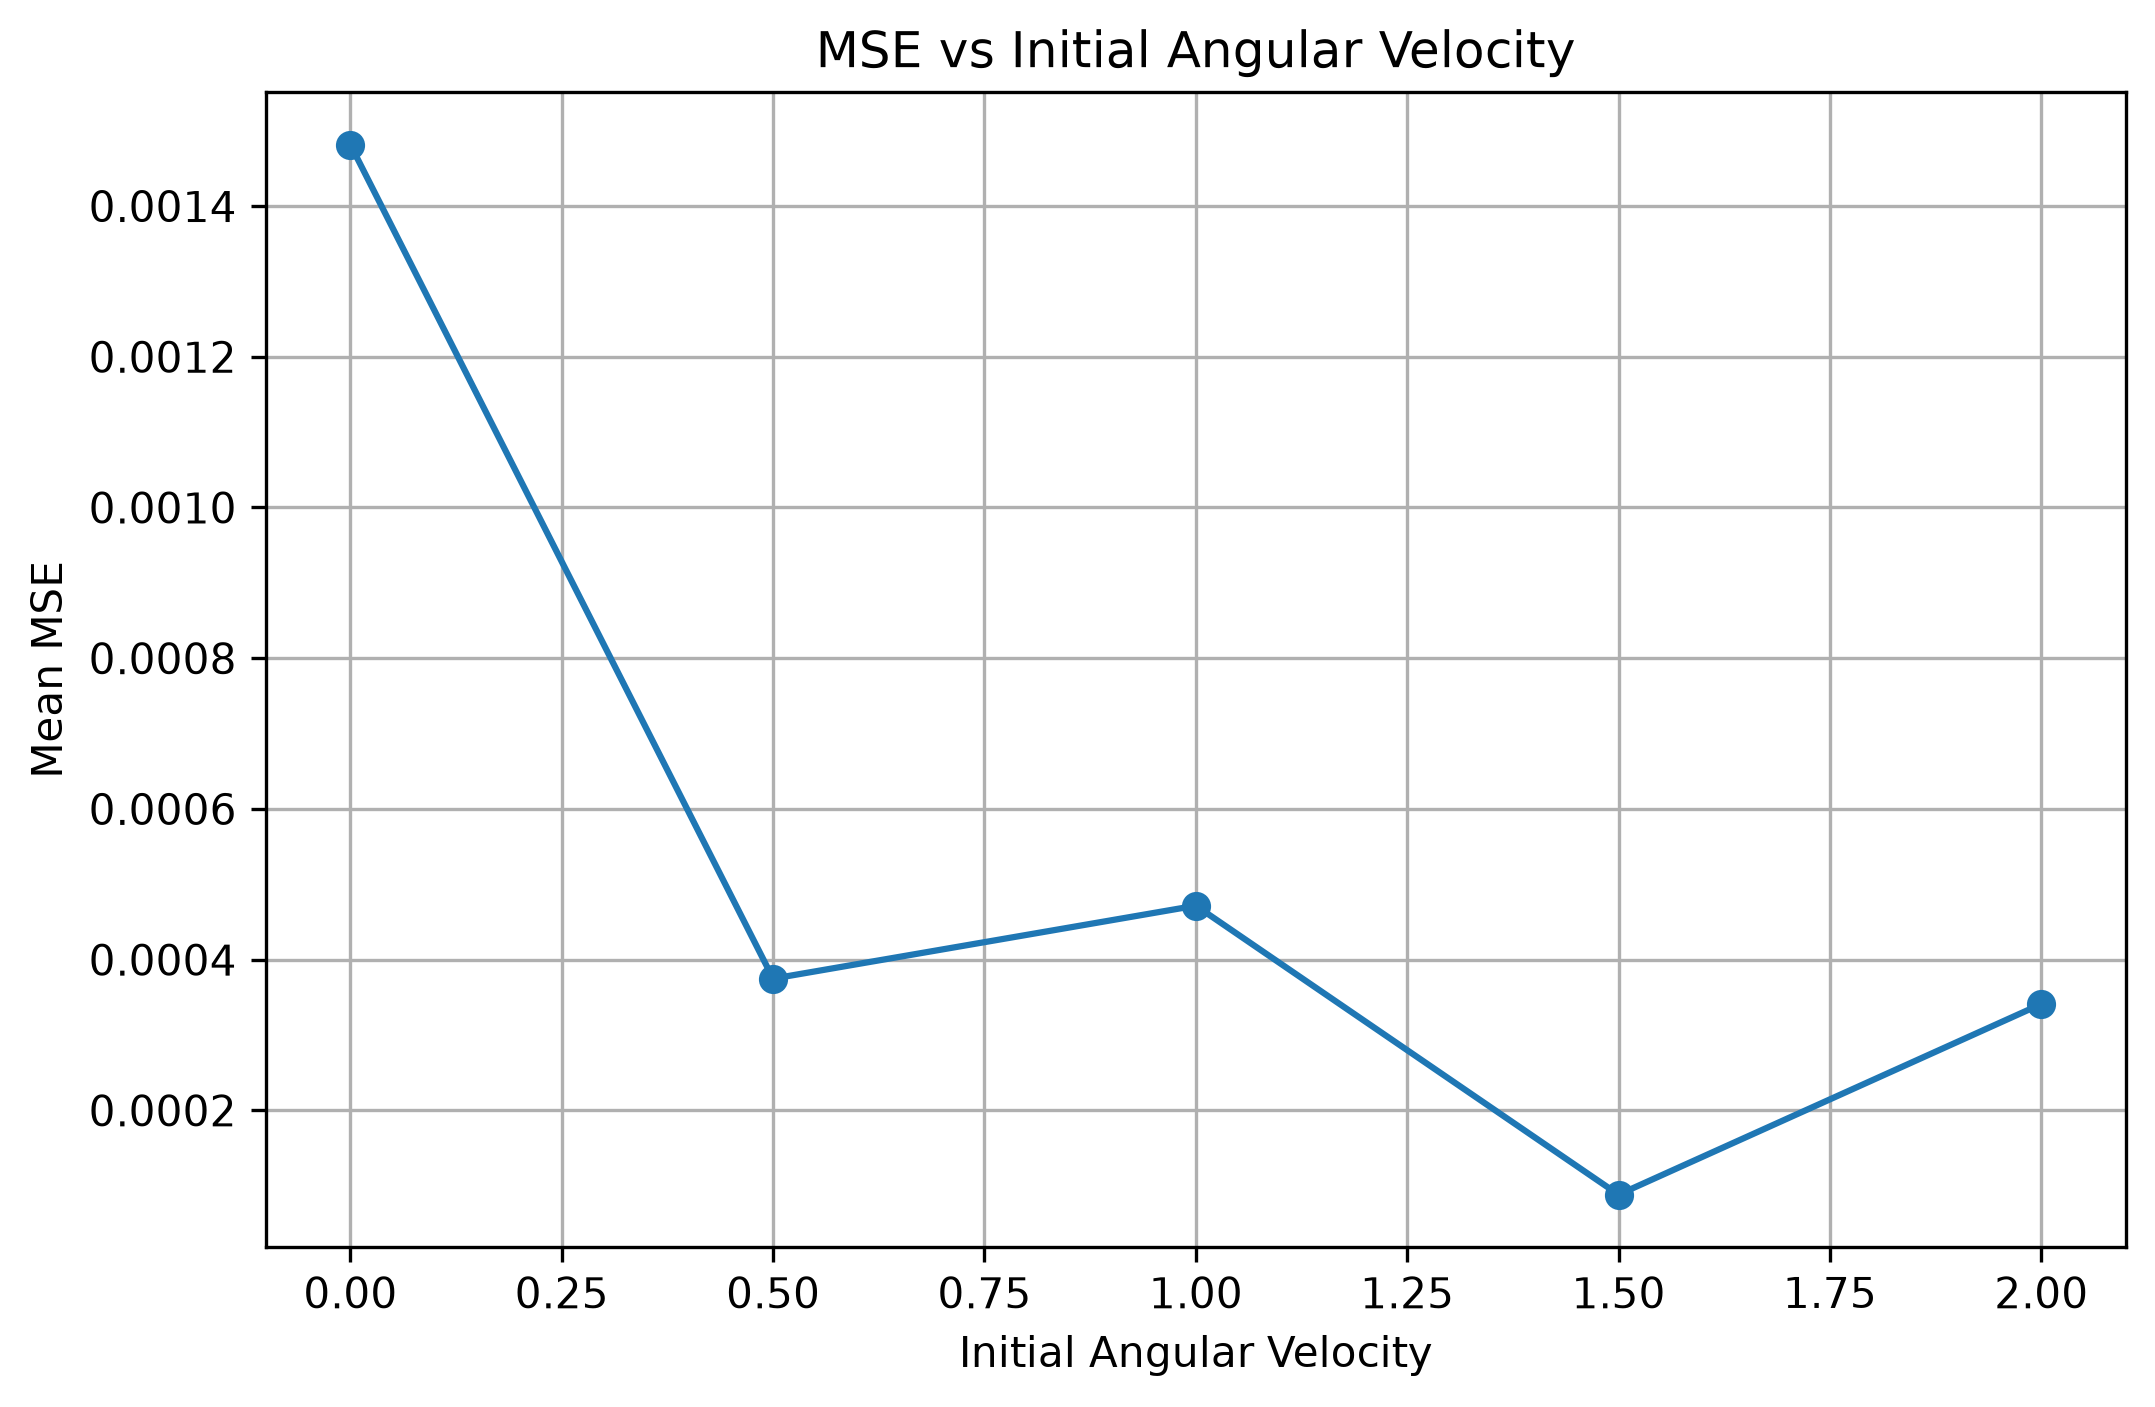
\includegraphics[width=0.8\textwidth]{figures/mse_vs_velocity.png}
\caption{\small Mean squared error (MSE) of the simple pendulum for different initial angular velocities ($\omega_0$). Results are averaged over five random seeds.}
\label{fig:mse_vs_velocity}
\end{figure}

The final sweep investigated the influence of the initial angular velocity. This experiment followed the same methodology as the previous sweeps, with five different initial velocities and five random seeds for each configuration. Figure 8 shows the average MSE for each initial angular velocity.

Increasing the initial angular velocity produces higher energy, larger oscillation amplitudes, and greater exploration of the nonlinear regime. Therefore, an initial hypothesis would be that larger initial velocities should result in higher prediction errors.

However, similarly to the initial angle sweep, no direct relationship between velocity and error was observed. The highest error occurred for $(\omega_0=0)$, with an MSE of $1.48\times10^{-3}$, whereas $(\omega_0=1.5)$ achieved an MSE of $8.8\times10^{-5}$. Therefore, increasing the initial angular velocity does not necessarily make the prediction problem more difficult.

A slight overall decrease in prediction error can be observed as the initial angular velocity increases, although this trend is not strictly monotonic. Intermediate values exhibit small fluctuations, suggesting that the effect of initial angular velocity on prediction accuracy is relatively weak compared with parameters such as simulation duration or gravitational acceleration.

Overall, the simple pendulum experiments show that prediction accuracy is influenced more strongly by the temporal characteristics of the generated trajectory than by the mere presence of nonlinear terms in the governing equation. Parameters that increase oscillation frequency or extend the prediction horizon have a much greater impact on performance than those that only increase the degree of nonlinearity.

\subsection{Double Pendulum}
The double pendulum represents the most complex dynamical system analysed in this study. Unlike the simple pendulum, it consists of two coupled pendulum arms, resulting in a system with two degrees of freedom and strongly nonlinear interactions between both components. The governing equations contain coupled nonlinear terms, making the resulting trajectories significantly more complex than those observed in previous systems.

For certain initial conditions, the double pendulum can exhibit chaotic behaviour \cite{strogatz2015nonlinear}, where small variations in the initial state may lead to substantially different trajectories over time \cite{lorenz1963deterministic}. This sensitivity to initial conditions represents an additional challenge for neural network-based modelling, as the objective is not only to approximate a given trajectory but also to generalise to unseen dynamical states.

To evaluate the performance of the neural network in this system, two types of experiments were performed. First, four parameter sweeps were conducted by varying the physical parameters of the system: the two pendulum lengths and the two initial angular positions. These experiments analyse how changes in the system configuration affect the prediction accuracy. Second, additional experiments were carried out to investigate the influence of sensitivity to initial conditions. In these experiments, small perturbations were introduced in the initial angle of the first pendulum to evaluate the ability of the model to generalise beyond the trajectory used during training.
\begin{figure}[htbp]
\centering
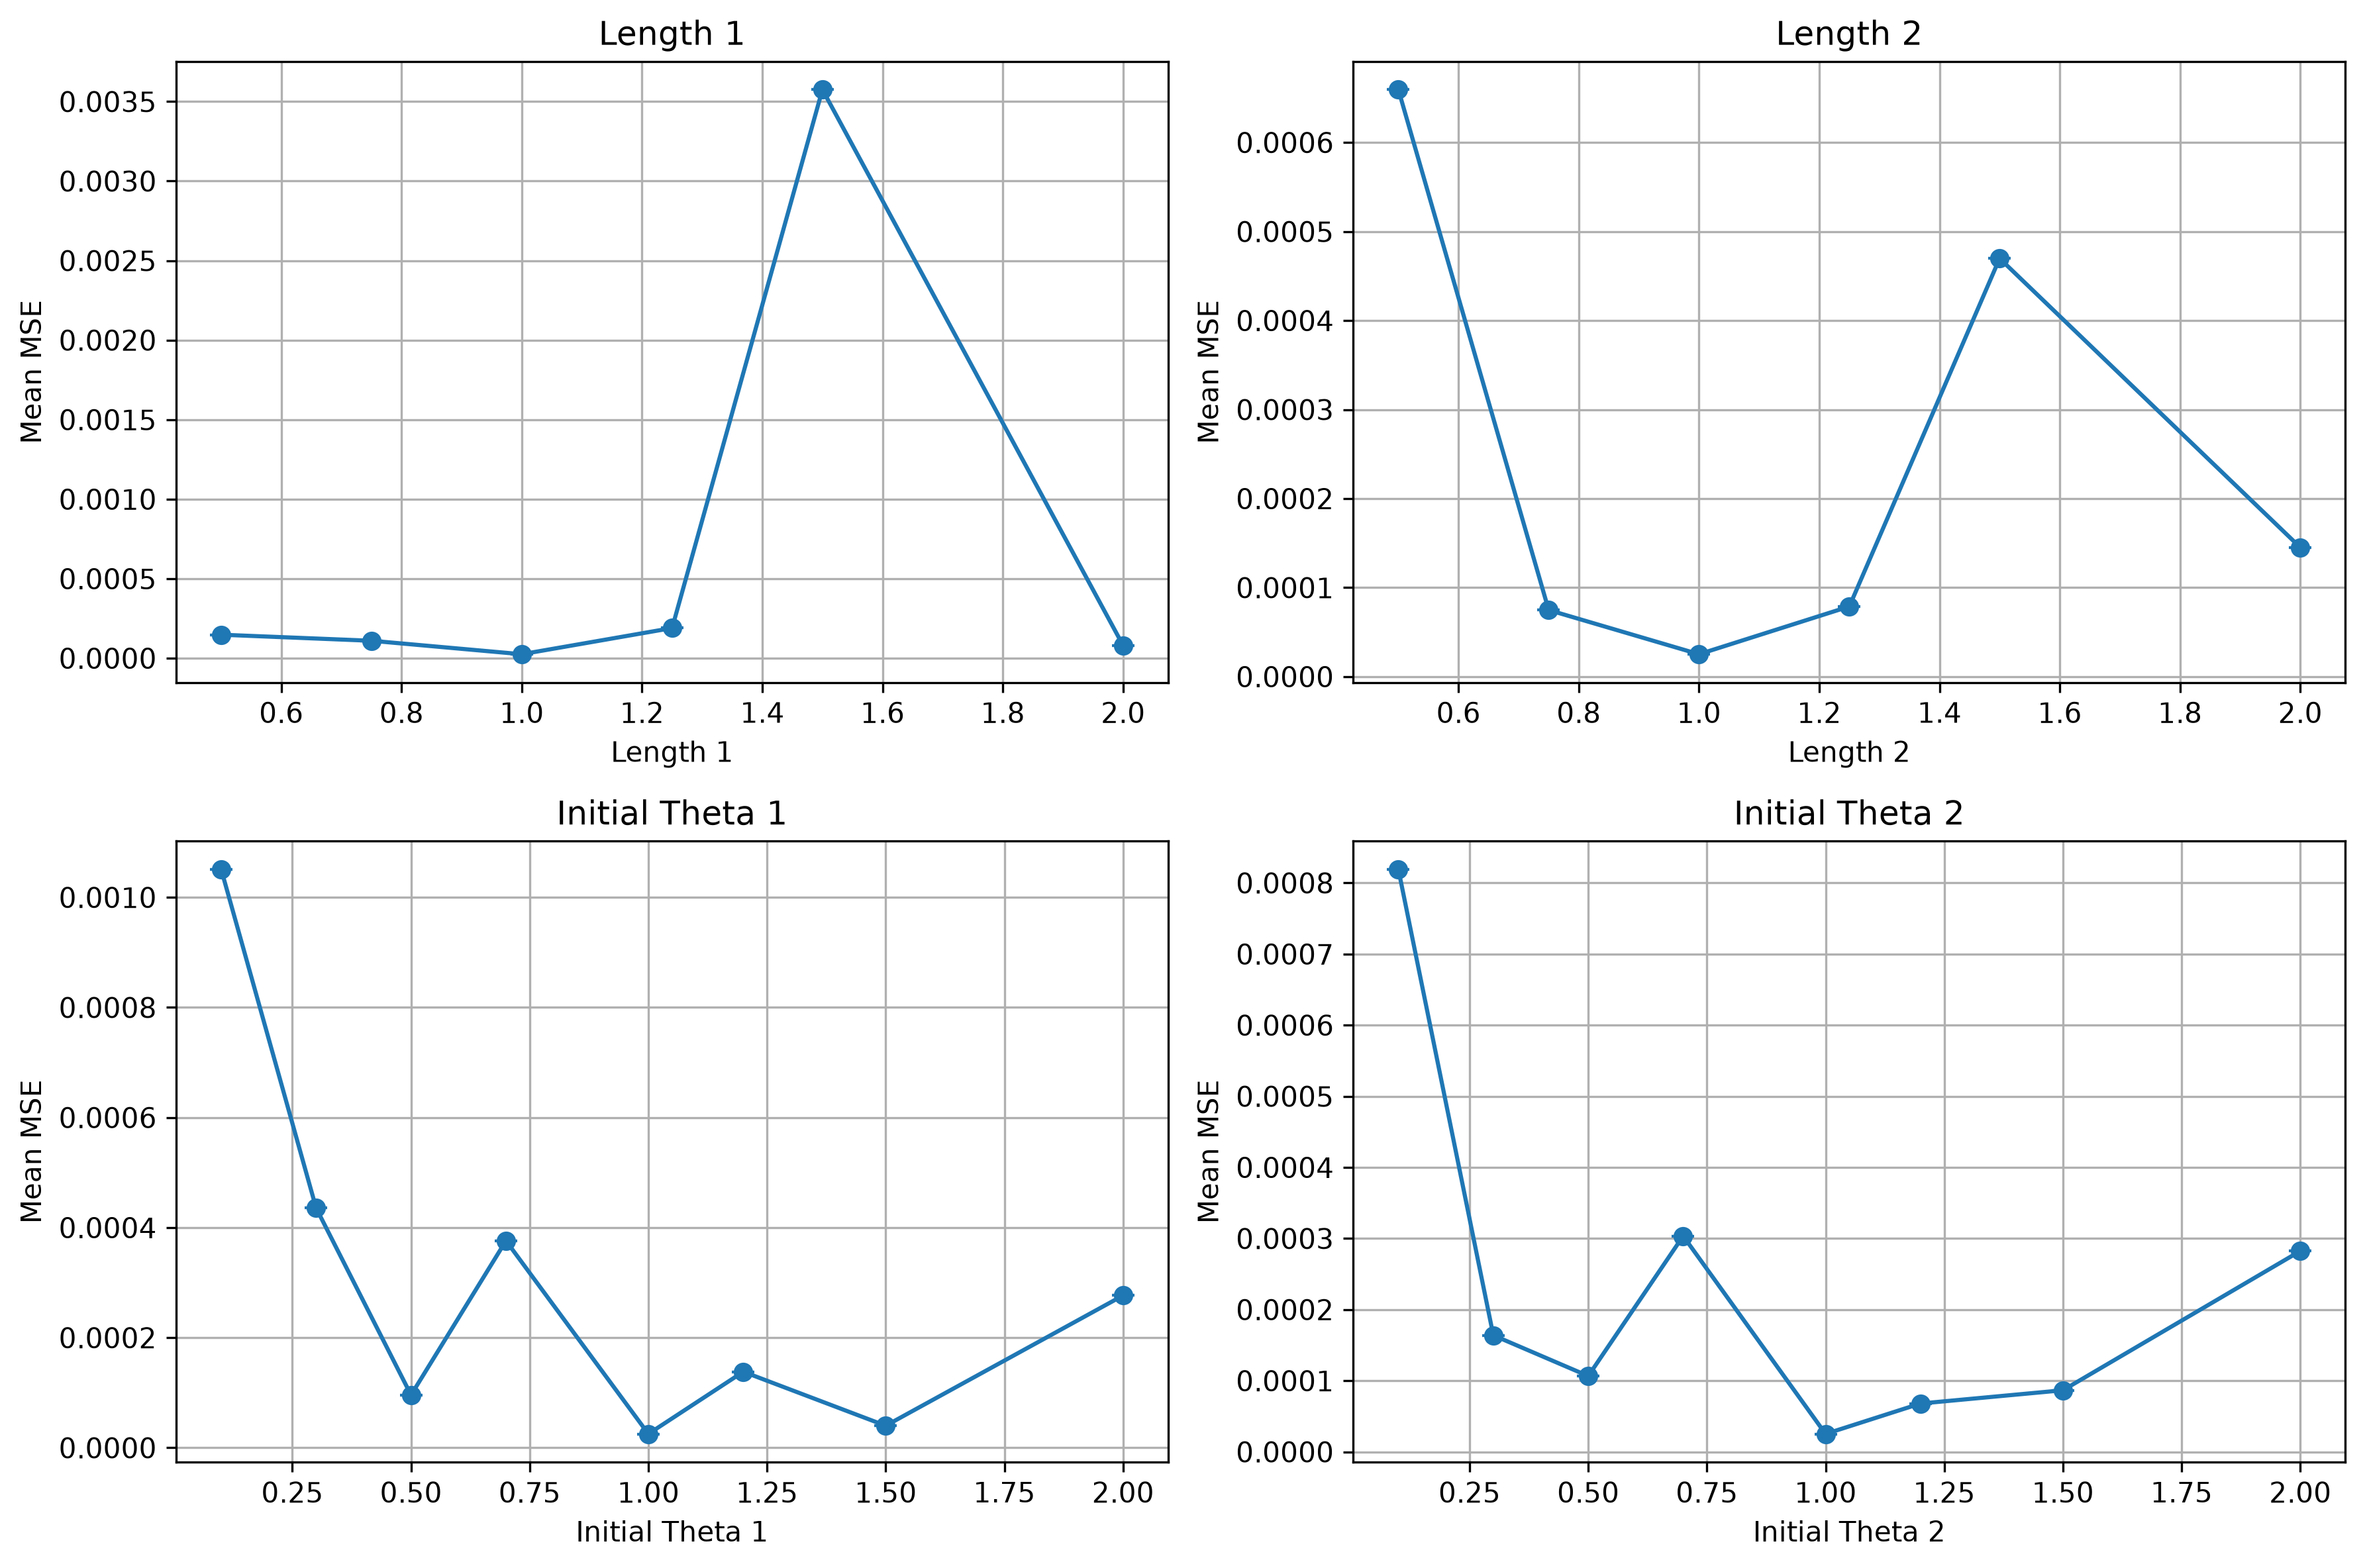
\includegraphics[width=0.8\textwidth]{figures/double_pendulum_parameter_sweeps.png}
\caption{\small Mean squared error (MSE) of the double pendulum for different physical parameter variations. The figure shows the prediction error obtained by varying the initial angular positions ($\theta_1$, $\theta_2$) and pendulum lengths ($L_1$, $L_2$).}
\label{fig:double_pendulum_parameter_sweeps}
\end{figure}

For the double pendulum system, four parameter sweeps were performed by independently varying the two pendulum lengths and the two initial angular positions. Each sweep consisted of six different parameter values evaluated using a single random seed. Therefore, unlike previous experiments, the reported MSE values do not represent averages over multiple training runs, but the result obtained for each individual configuration. The objective of these experiments was to analyse how changes in the physical parameters affect the ability of the neural network to approximate the coupled nonlinear dynamics of the system.

The first two experiments investigated the influence of the pendulum lengths. Figure 9 shows the MSE obtained for the $L_1$ and $L_2$ sweeps. In both cases, no clear monotonic relationship between the length and the prediction error can be observed. Interestingly, the lowest error in both experiments corresponds to the reference configuration, where both lengths are equal to 1. For this case, the network achieved an MSE of $2.52\times10^{-5}$, indicating that this configuration generates a trajectory that is particularly suitable for approximation.

For the $L_1$ sweep, most configurations maintained low errors, with MSE values below $2\times10^{-4}$. However, when $(L_1=1.5)$, the error increased significantly, reaching an MSE of $3.58\times10^{-3}$. This result shows that increasing the length of the first pendulum does not directly translate into higher prediction error. Instead, specific length configurations can generate more challenging dynamics for the neural network.

A possible explanation is that modifying $L_1$ changes the coupling between the two pendulums. Unlike the simple pendulum, where the length mainly determines the oscillation frequency, the double pendulum contains two interacting degrees of freedom. Changing the first pendulum length affects the energy transfer between both pendulums and can modify the resulting trajectory complexity. Therefore, certain configurations may produce less regular temporal patterns that are harder for the neural network to approximate.

The $L_2$ sweep showed a similar but less pronounced behaviour. The errors remained low for most configurations, although the smallest length value, $(L_2=0.5)$, produced the highest MSE of $6.59\times10^{-4}$. Again, the reference configuration $(L_2=1)$ achieved the lowest error. Since the second pendulum is influenced by the motion of the first one but does not directly control the entire system dynamics, variations in $L_2$ appear to have a smaller impact on the prediction difficulty.

The influence of the initial conditions was analysed through the $\theta_1$ and $\theta_2$ sweeps. As in the length experiments, the lowest error was obtained for the reference configuration, with $(\theta_1=\theta_2=1)$ rad resulting in an MSE of $2.52\times10^{-5}$. However, no monotonic relationship between the initial angle and the prediction error was observed.

For the $\theta_1$ sweep, the largest error was obtained for an initial angle of 0.1 rad, with an MSE of $1.05\times10^{-3}$, while several larger angles achieved lower errors. Similarly, the $\theta_2$ sweep showed variations between different initial angles, but without a clear tendency for the error to increase as the initial displacement increased.

This behaviour differs from what would be expected if the difficulty depended only on the degree of nonlinearity. For small angles, the simple pendulum approximation
\begin{equation}
    \sin(\theta)\approx\theta
\end{equation}

is valid, resulting in a system closer to a linear oscillator. For larger angles, this approximation becomes invalid and nonlinear effects become more significant. However, the results indicate that increasing nonlinearity alone is not enough to substantially degrade the performance of the neural network.

Overall, the four parameter sweeps show that the difficulty of learning double pendulum dynamics is not determined by a single physical parameter. Instead, the prediction error depends on the complexity of the resulting trajectory and on the interaction between the two coupled degrees of freedom. Most configurations remained within the approximation capabilities of the neural network, while specific combinations of parameters produced more complex dynamics and increased prediction errors. These results suggest that trajectory complexity is a more relevant factor than the magnitude of an individual physical parameter when evaluating the learning difficulty of nonlinear dynamical systems.

After analysing the influence of the physical parameters of the double pendulum, an additional experiment was performed to study one of the main characteristics of chaotic systems: sensitivity to initial conditions.

Unlike the previous sweeps, the objective of this experiment was not to determine how a parameter affects the prediction error of the neural network. Since each trajectory was trained and evaluated independently, similar prediction errors are expected for different initial conditions. Instead, this experiment aimed to analyse whether small variations in the initial state lead to significantly different system evolutions.
All physical parameters were kept constant:
\begin{equation}
    m_1=m_2=1,\quad L_1=L_2=1,\quad g=9.81
\end{equation}

with initial conditions:
\begin{equation}
    \theta_2=1.0,\quad \omega_1=\omega_2=0
\end{equation}

The initial angle of the first pendulum was modified as:
\begin{equation}
    \theta_1={1.0,1.0001,1.001,1.01,1.1}
\end{equation}

These values represent increasingly larger perturbations around the same initial configuration. Each case was simulated and approximated by an independent neural network with the same architecture and training parameters.
\begin{table}[htbp]
\centering
\small
\begin{tabular}{ccc}
\toprule
Initial Angle & 
MSE & $R^2$ \\
\midrule
1.0 & 0.001191 & 0.997872 \\
1.0001 & 0.000508 & 0.999064 \\
1.001 & 0.000684 & 0.998787 \\
1.01 & 0.000429 & 0.999253 \\
1.1 & 0.002033 & 0.996512 \\

\bottomrule
\end{tabular}
\caption{Prediction performance of the double pendulum for different initial values of $\theta_1$. Each row corresponds to an independent experiment performed with a single random seed.}
\label{tab:double_pendulum_experiment}
\end{table}

The obtained prediction metrics are shown in Table 2. All configurations achieved similar performance, with $R^2$ values above 0.996. No clear relationship between the initial angle perturbation and the prediction error was observed. This result is expected, as each neural network learns its corresponding trajectory independently. Therefore, the differences in MSE do not represent the divergence between trajectories, but rather small variations in the approximation process.

To analyse the chaotic behaviour of the system, the difference between trajectories generated from different initial conditions was calculated:

\begin{equation}
    |\Delta\theta_1(t)|=|\theta_{1,a}(t)-\theta_{1,b}(t)|
\end{equation}

\begin{figure}[htbp]
\centering
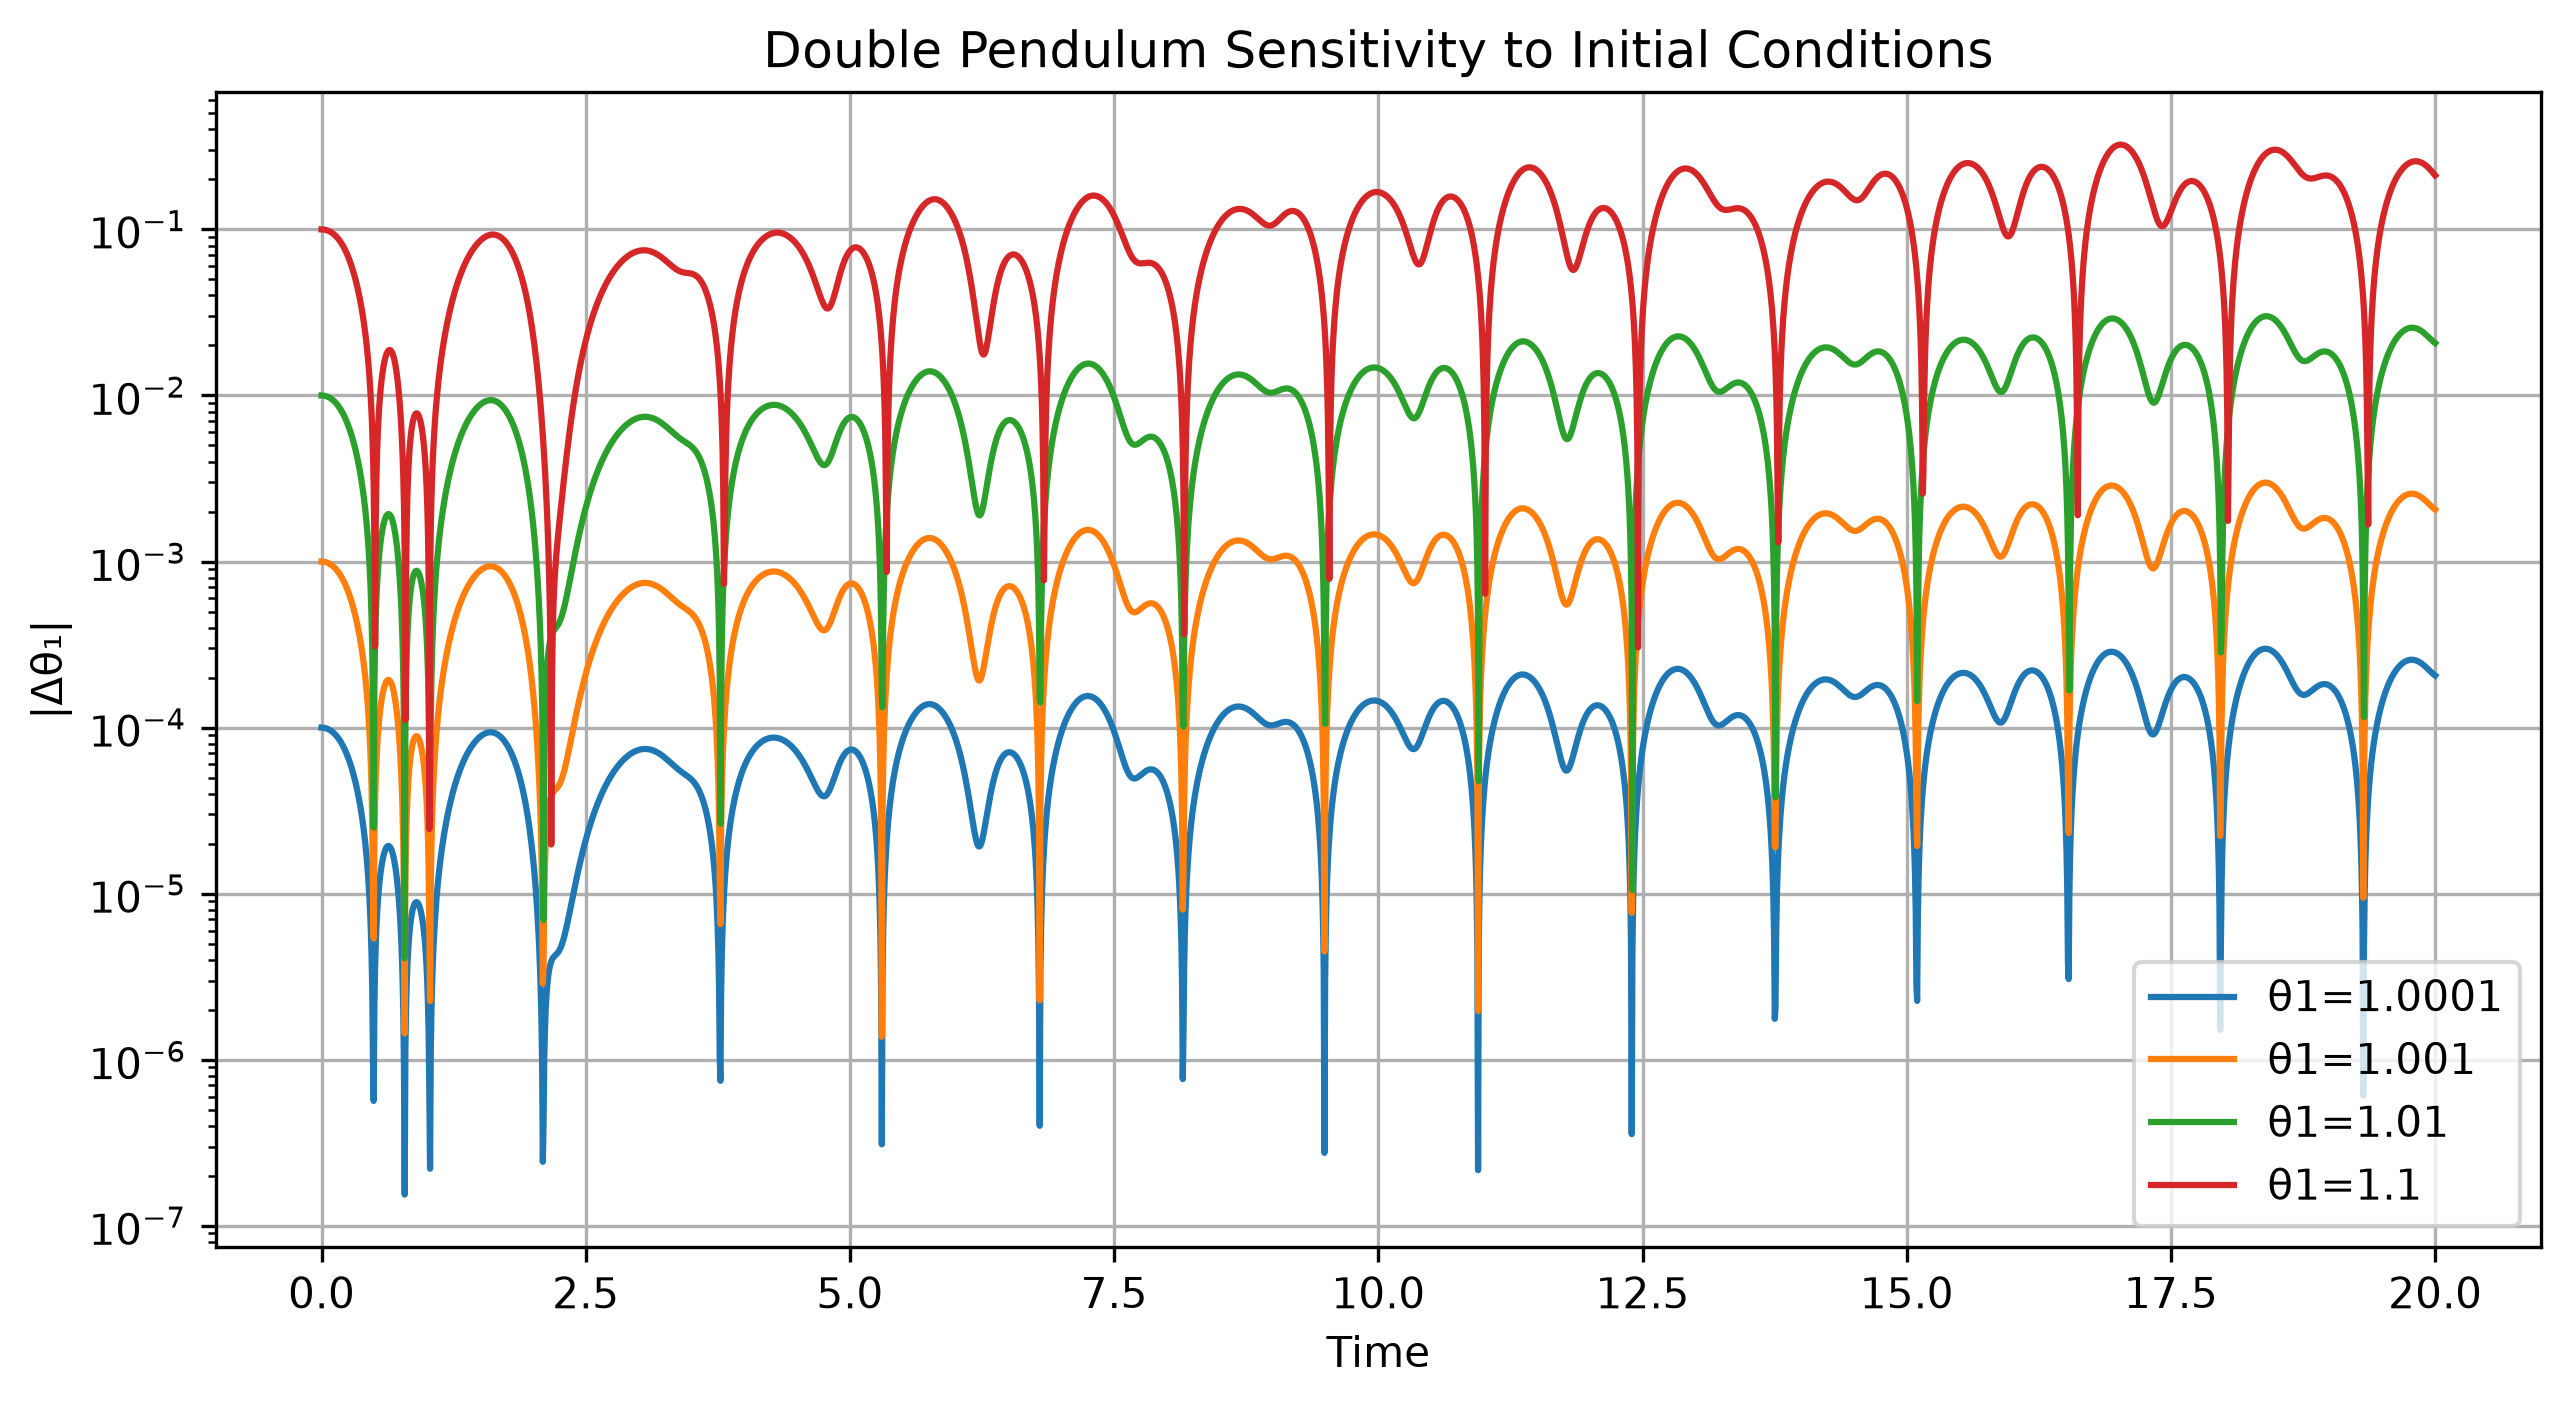
\includegraphics[width=0.8\textwidth]{figures/sensitivity_theta1.png}
\caption{\small Evolution of the absolute angular difference $|\Delta\theta_1|$ for four double pendulum trajectories with slightly different initial conditions.}
\label{fig:sensitivity_theta1}
\end{figure}

Figure 10 shows the evolution of this angular difference over time for the tested initial conditions. At the beginning of the simulation, the trajectories remain almost identical due to their extremely similar initial states. However, as time increases, the difference between them grows significantly.
This divergence illustrates the sensitivity to initial conditions characteristic of chaotic systems \cite{lorenz1963deterministic}. Even small perturbations that are negligible at the beginning can lead to substantially different future states. Consequently, two trajectories generated from initial conditions such as $(\theta_1=1.0)$ and $(\theta_1=1.0001)$ may evolve into noticeably different motions despite starting from almost identical configurations.
This observation is important for neural network modelling of chaotic systems. A network trained on a single trajectory may accurately reproduce that specific evolution, but this does not necessarily imply that it has learned the underlying dynamics of the system. The strong dependence on the initial state suggests that generalizing to nearby but unseen trajectories represents a more challenging task.
For this reason, the following experiment evaluates the ability of the neural network to predict trajectories generated from different initial conditions after being trained only on a single reference trajectory.
\begin{figure}[htbp]
\centering
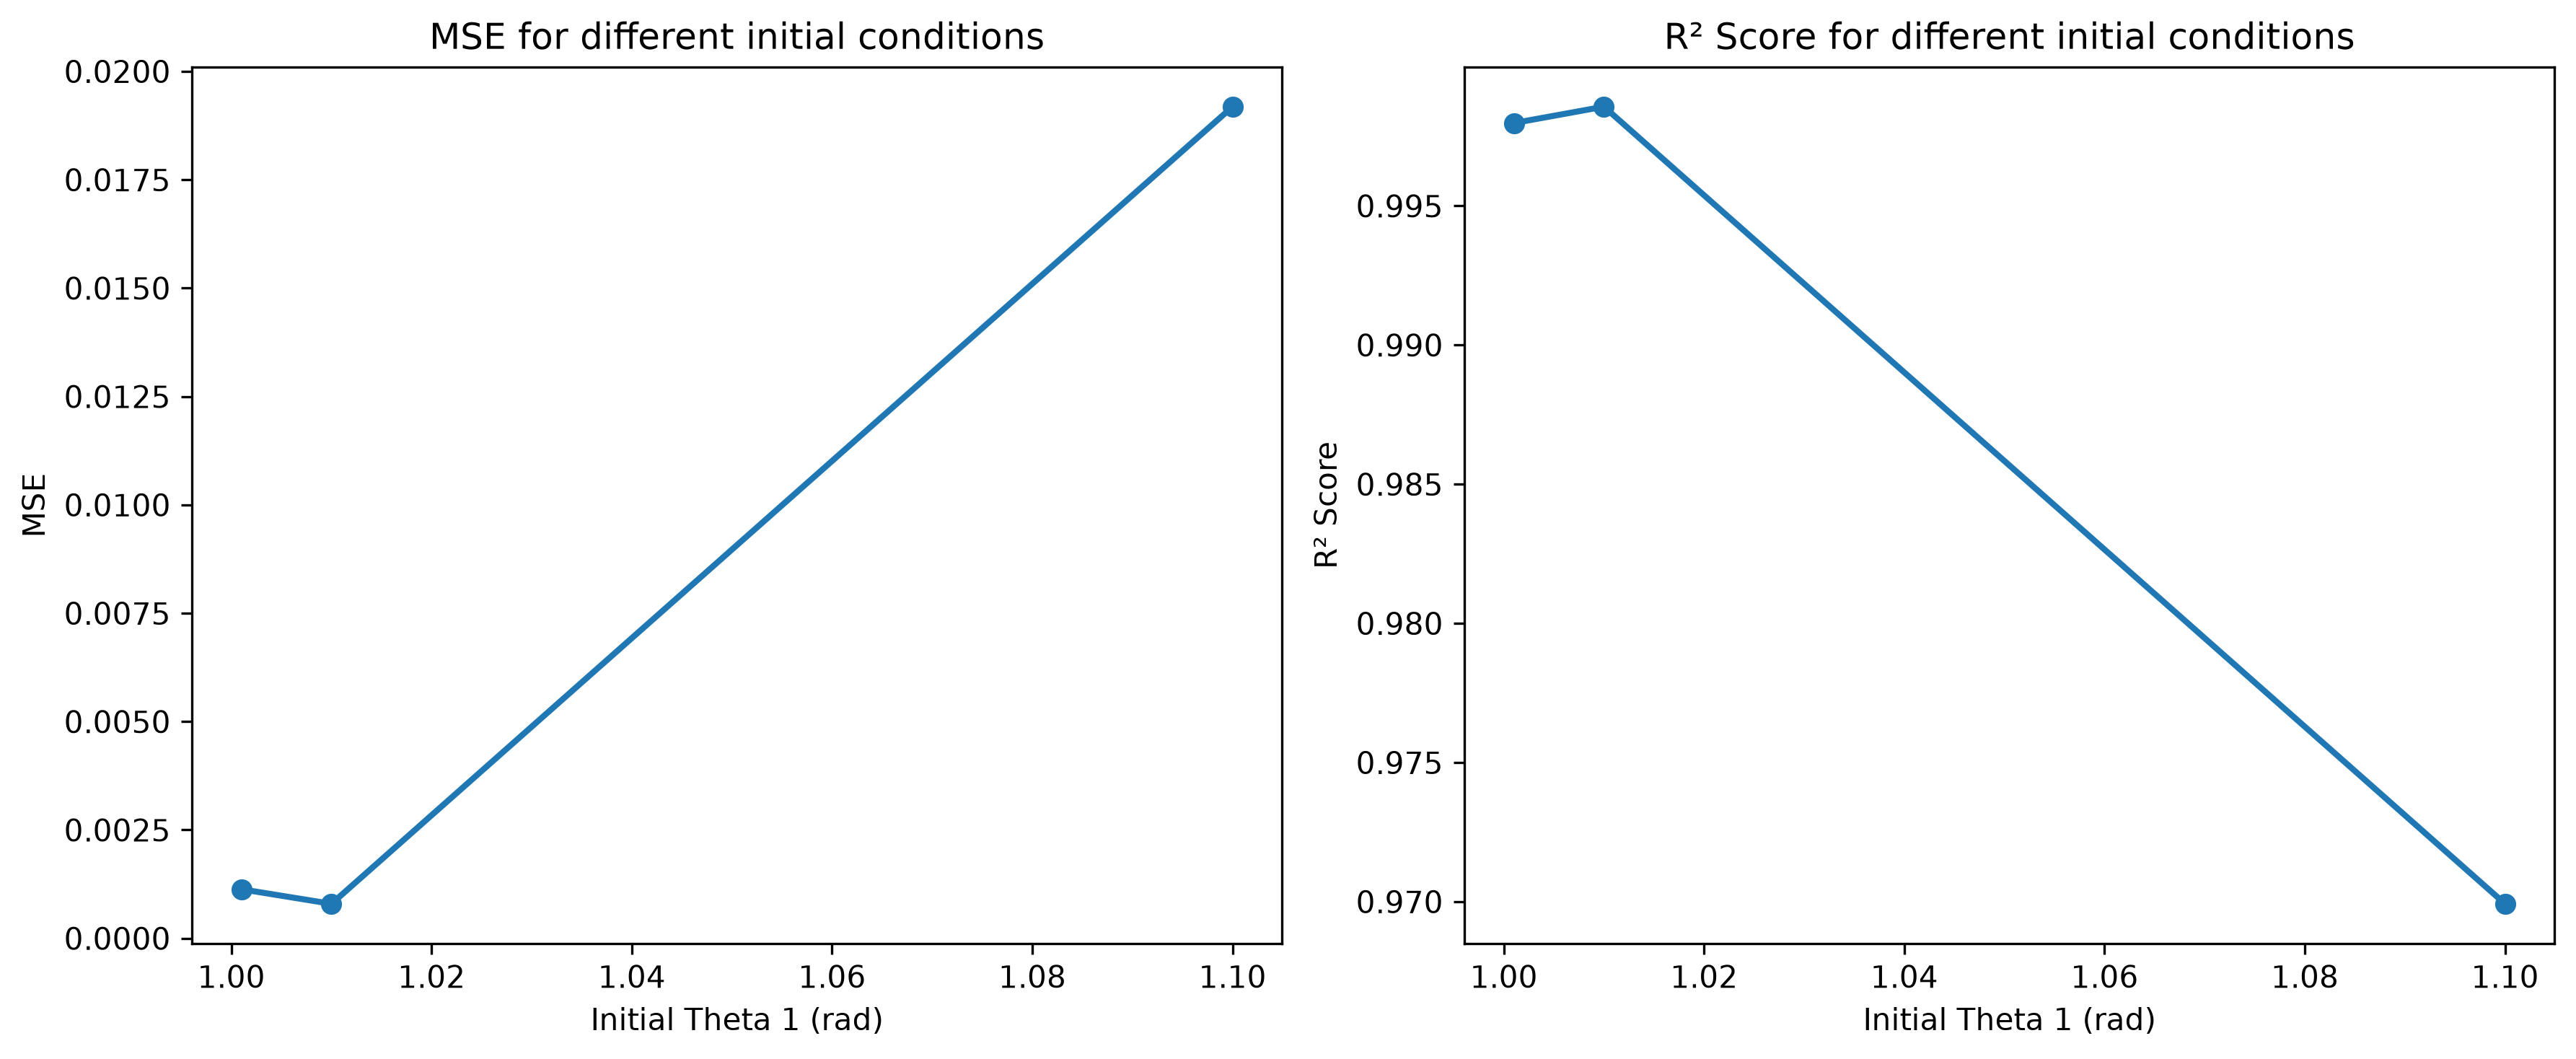
\includegraphics[width=0.8\textwidth]{figures/theta1_chaos_test_results.png}
\caption{\small Generalization performance of the neural network trained with an initial angle of $\theta_1 = 1.0$. The left panel shows the mean squared error (MSE), while the right panel shows the coefficient of determination ($R^2$), evaluated for different initial values of $\theta_1$.}
\label{fig:theta1_chaos_test_results}
\end{figure}


Following the previous analysis of sensitivity to initial conditions, a final experiment was performed to evaluate the ability of the neural network to generalize between nearby chaotic trajectories.

In contrast with the previous experiment, where each initial condition was trained and evaluated independently, in this case the neural network was trained using only a single trajectory with:
\begin{equation}
    \theta_1=1.0
\end{equation}

while the evaluation was performed on trajectories generated from different initial conditions:
\begin{equation}
    \theta_1={1.001,1.01,1.1}
\end{equation}

All remaining physical parameters were kept constant.

The results are shown in Figure 11. For small perturbations of the initial condition, the network maintains high prediction accuracy. The cases $(\theta_1=1.001)$ and $(\theta_1=1.01)$ achieve $R^2$ values of 0.998 and 0.999 respectively, indicating that the predicted trajectories remain close to the reference solution.

However, when the initial angle is changed to $(\theta_1=1.1)$, the prediction error increases significantly, reaching an MSE of $1.92\times10^{-2}$ and reducing the $R^2$ score to 0.9699. This degradation occurs because the evaluated trajectory progressively diverges from the trajectory used during training due to the sensitivity to initial conditions of the double pendulum.

These results highlight an important limitation of neural networks applied to chaotic systems. Although the model can accurately approximate a specific trajectory, learning one solution does not guarantee accurate prediction of other nearby trajectories. The chaotic nature of the system causes small differences in the initial state to produce different future evolutions, limiting the generalization capability of the model.

Overall, the double pendulum experiments show that neural networks can accurately approximate individual nonlinear trajectories. However, the results from the chaos test demonstrate a fundamental limitation: accurate prediction requires the model to be trained on the specific dynamical regime it is expected to reproduce. Small differences in initial conditions can lead to significant prediction errors due to the chaotic nature of the system.
